\documentclass[oneside, a4paper, 11pt, ]{report}
\usepackage{graphicx}
\usepackage{amssymb}
\usepackage{amsmath}
\usepackage{algorithm}
\usepackage[noend]{algpseudocode}}
\usepackage{braket}
\usepackage{mathrsfs}
\usepackage{appendix}
\linespread{1.5}
\usepackage{algorithm}
\usepackage[noend]{algpseudocode}
\usepackage[margin=1.1in]{geometry}
\usepackage{lineno}
\usepackage{bbold}
\usepackage{epstopdf}
\usepackage{fancyhdr}
\usepackage{rotating}
\usepackage{afterpage,lscape}
\usepackage{draftwatermark}
\usepackage{hyperref}
\usepackage{geometry}
\usepackage{float}
  \geometry{
  a4paper,
  total={210mm,297mm},
  left=40mm,
  right=15mm,
  top=20mm,
  bottom=20mm,
  }

\hypersetup{
    colorlinks,
    citecolor=blue,
    filecolor=blue,
    linkcolor=blue,
    urlcolor=blue
}



%\SetWatermarkText{DRAFT}
%\normalfont\SetWatermarkScale{7}

\title{\title} % Defines the thesis title - don't touch this

\begin{document}


%\pagestyle{fancyplain}
%\fancyhead[LE, RO]{}
%\fancyhead[LE, RO]{\slshape \rightmark}
%\fancyhead[RE, LO]{\slshape \leftmark}
\fancyfoot[C]{\thepage}
\renewcommand{\headrulewidth}{0.4pt}
\newcommand{\HRule}{\rule{\linewidth}{0.5mm}} % New command to make the lines in the title page


%%%%%%%%%%%%%%%%%%%%%%%%%%%%%%%%%%%%%%%%%%%%%%%%
%Title Page
%%%%%%%%%%%%%%%%%%%%%%%%%%%%%%%%%%%%%%%%%%%%%%%%

\begin{titlepage}
\begin{center}

\textsc{\LARGE Brunel University London}\\[0.5cm] % University name

\includegraphics[scale=0.5]{Figures/brunelshield.png} \\[0.5cm]
\textsc{\Large Doctoral Thesis}\\[0.5cm] % Thesis type

\HRule \\[0.4cm] % Horizontal line
{\huge \bfseries A scalable datastore and analytic platform for real-time monitoring of scientific infrastructure}\\[0.3cm] 
\HRule \\[1.5cm] % Horizontal line
 
\begin{minipage}{0.4\textwidth}
\begin{flushleft} \large
\emph{Author:}\\
Uthayanath Suthakar 
\end{flushleft}
\end{minipage}
\begin{minipage}{0.4\textwidth}
\begin{flushright} \large
\emph{Supervisors:} \\
Dr. David Rayn Smith \\
Prof. Akram Khan
\end{flushright}
\end{minipage}\\[2cm]

\large \textit{ A dissertation submitted to Brunel University\\ in accordance with the requirements\\ for award of the degree of Doctor of Philosophy}\\[0.3cm] 
\textit{in}\\[0.4cm]
\textit{the Faculty of Electronic and Computer Engineering\\\ Centre for Sensors \& Instrumentation} \\

\vspace*{10mm}
{\large \today}\\[4cm]
%\vspace*{-12mm}

\end{center}

\end{titlepage}

\pagestyle{empty}

%%%%%%%%%%%%%%%%%%%%%%%%%%%%%%%%%%%%%%%%%%%%%%%%
%Declaration
%%%%%%%%%%%%%%%%%%%%%%%%%%%%%%%%%%%%%%%%%%%%%%%%

\newpage

\begin{declaration}
\begin{center}
 \begin{large}
\textbf{Declaration of Authorship}
\end{large}
\end{center}

\noindent I, Uthayanath Suthakar, declare that the work in this dissertation was carried out in accordance with the requirements of the University's Regulations and Code of Practice for Research Degree Programmes and that it has not been submitted for any other academic award. Except where indicated by specific reference in the text, the work is the candidate's own work. Work done in collaboration with, or with the assistance of, others, is indicated as such. Any views expressed in the dissertation are those of the author.\\

\begin{center}
SIGNED: $...............................................................$  DATE: $...................................$

(Signature of student)

\vspace{12pt}
\end{center}
\null\vfill
\end{declaration}

\clearpage

%%%%%%%%%%%%%%%%%%%%%%%%%%%%%%%%%%%%%%%%%%%%%%%%
%Quotes
%%%%%%%%%%%%%%%%%%%%%%%%%%%%%%%%%%%%%%%%%%%%%%%%

\pagestyle{empty} % No headers or footers for the following pages

\null\vfill % Add some space to move the quote down the page a bit

%\textit{``Real courage is when you know you're licked before you begin, but you begin anyway and see it through no matter what."}

\begin{flushright}
%Harper Lee, To Kill a Mockingbird
\end{flushright}

\vfill\vfill\vfill\vfill\vfill\vfill\null % Add some space at the bottom to position the quote just right

\clearpage % Start a new page

%%%%%%%%%%%%%%%%%%%%%%%%%%%%%%%%%%%%%%%%%%%%%%%%
%Abstract
%%%%%%%%%%%%%%%%%%%%%%%%%%%%%%%%%%%%%%%%%%%%%%%%

\begin{abstract}


\end{abstract} 

\clearpage

%%%%%%%%%%%%%%%%%%%%%%%%%%%%%%%%%%%%%%%%%%%%%%%%
%Acknowledgements
%%%%%%%%%%%%%%%%%%%%%%%%%%%%%%%%%%%%%%%%%%%%%%%%

\acknowledgements{\addtocontents{toc}{\vspace{1em}} % Add a gap in the Contents, for aesthetics

The acknowledgements and the people to thank go here\ldots
}
\clearpage % Start a new page

% Insert biography and acknowledgements code here

\pagestyle{empty}

%%%%%%%%%%%%%%%%%%%%%%%%%%%%%%%%%%%%%%%%%%%%%%%%
%Declaration
%%%%%%%%%%%%%%%%%%%%%%%%%%%%%%%%%%%%%%%%%%%%%%%%

\newpage

\begin{Publications}
\begin{center}
 \begin{large}
\textbf{List of Publications}
\end{large}
\end{center}

\noindent The following papers have been accepted / to be submitted for publication as a direct or indirect result of the research discussed in this thesis.\\

\null\vfill
\end{Publications}

\clearpage

\pagestyle{fancyplain}

\setcounter{page}{1}
\setcounter{secnumdepth}{3}
\pagenumbering{roman}

\tableofcontents
\listoffigures
\listoftables
\clearpage

%\linenumbers

%\pagestyle{fancyplain}
\pagenumbering{arabic}
%\setcounter{page}{1}

\clearpage

%\linespread{1.3} %%line spaceing 1.5

%\fancyhead[le,ro]{\slshape \rightmark} %le and ro were in capitals
%\fancyhead[lo,re]{\slshape \leftmark}

%\addcontentsline{toc}{chapter}{Introduction}
\chapter{Introduction} \label{introduction}

%\section{Motivations} \label{Motivations}

\section{Motivations} \label{motivations}
\section{Methodology} \label{methodology}
\section{Major Contributions to Knowledge} \label{contribution-to-know}
\section{Thesis Organization} \label{thesis-org}






%\addcontentsline{toc}{chapter}{Review of Literature}
\chapter{Review of Literature} \label{review-of-literature}

\section{Architecture} \label{Technology}

\subsection{Introduction} \label{subsec-lr-arc-intro}
\subsection{Summary} \label{subsec-lr-arc-summ}

\section{Technology} \label{Technology}

\subsection{Introduction} \label{subsec-lr-tech-intro}

The aim of this document is to review some of the state-of-the-art technology that can be used to architect the monitoring system for storing and handling big datasets and performing real-time analytics on them. The proposed architecture will consist of three layers: the batch layer, serving layer and speed layer.\\

\subsection{Batch Layer} \label{subsec-lr-batchlayer}

\subsubsection{Introduction} \label{subsubsec-lr-batchlayer-intro}
A batch layer is required to store constantly growing big data and for historical data analysis that is used to identify patterns such as job failures, popular data, busy sites and so forth.  Many individuals consider Hadoop as the de facto framework for analysing big data. However, there are many technologies available in the distributed system such as the Internet that go beyond MapReduce, a programming model for processing big data that was introduced by Google \cite{mr-com} . In this chapter an attempt will be made to review such technologies.\\

\subsubsection{Apache Hadoop- MapReduce and HDFS} \label{subsubsec-lr-batchlayer-mr}
The Hadoop stack has been used for many research and commercial products. It has gone through rigorous implementation and testing, which makes it robust. There are many Hadoop ecosystems and distributions, but in order to make this review relevant to the proposed layer, the MapReduce and Hadoop Distributed File System (HDFS) will be analysed. MapReduce is a programming model that was designed to remove the complexity of processing data that are geographically scattered around the distributed infrastructure \cite{mr-com,mr-data}. It hides the complexity of computing in parallel, load balancing and fault tolerance over a large range of inter-connected machines from developers.\\

There are two simple parallel methods; map and reduce are predefined in the MapReduce programming model and are user-specified methods, so users have control over how the data should be processed \cite{mr-data}. Hadoop was designed taking into account that moving computing to where the data reside is better than vice versa as it will reduce bottlenecks in the network, especially when the data that are being transferred are at the rate of terabytes-to-petabytes \cite{mr-com}. Therefore, map and reduce jobs will be allocated to where the data reside, which will be scheduled by JobTask Manager as shown in Figure \ref{fig-map-reduce}. The data will be read from the local disk (file system); mapped, with all records being independently processed and key/value pairs assigned; intermediate results are stored to the local disk and they are shuffled (transferred to where the reduce jobs are located); and reduced, so that records with identical keys are processed together and the output is written back to the disk (this output could be an input to another MapReduce job) \cite{mr-com}. Fault tolerance in MapReduce is supported by periodically checking the heartbeat of the worker nodes, master failures can be protected against by using check-pointing, an approach used to enable applications to recover from failure.\\

\begin{figure}[H]
\centering
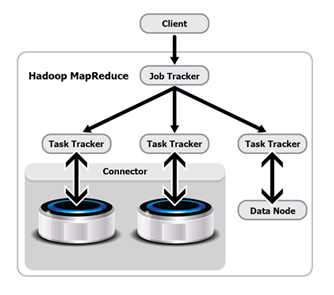
\includegraphics[width=0.5\textwidth]{Figures/map-reduce.png}
\caption{Hadoop Architecture}\label{fig-map-reduce}
\end{figure}

The MapReduce framework is built on HDFS and executes I/O operations on it. The HDFS guarantees: scalability on commodity hardware, fault tolerance, high throughput, load balance, data integrity and portability \cite{intro-hdfs}. It employs master-slave architecture, which is prone to single point failure. However, it facilitates failover to the standby server but this is prone to downtime. Data are replicated across disk nodes for load balancing, fault tolerance and high availability \cite{intro-hdfs}.

\subsubsection{Stratosphere} \label{subsubsec-lr-batchlayer-stratosphere}
Stratosphere extends the MapReduce model as discussed in section \ref{subsubsec-lr-batchlayer-mr} with new operators such as union, iterate, join, cross and cogroup as shown in Fig. 2. All operators will start working in the memory and when there isn’t enough memory then the rest of the data will be processed from the disk. The principal concept in Stratosphere is Parallelisation contracts (PACTs), which categorises three types: input contract, which suggests how inputs to compute nodes are structured; user function, which enables developers to program how to transform from inputs to outputs and output contract, which offers compiler hints to achieve performance improvement (4). PACTs are data processing objects in the data flow. Input data go through nodes for transformation, computation, and optimisation in parallel. Stratosphere distributes the resource manager and execution engine called Nephele, which utilises a master-slaves structure where the single master node receives a job graph from the upper layer as grounds to apply for resources by communicating with the resource administrative unit that is used to manage the computing resources of slave nodes (4). When adequate resources are available for a certain job, the master node distributes tasks to slave nodes and keeps track of their progress such as initialisation, running, completion and so forth.

\begin{figure}[H]
\centering
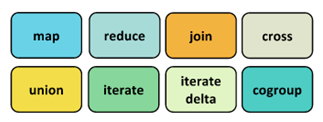
\includegraphics[width=0.5\textwidth]{Figures/stratosphere.png}
\caption{Stratosphere Operators}\label{fig-stratosphere}
\end{figure}

\subsubsection{Apache Spark} \label{subsubsec-lr-batchlayer-spark}
Apache Spark is an in-memory distributed computing framework (5, 6). It provides a general programming model supporting iterative classes of algorithms, interactive applications and algorithms containing common operators such as Map, Reduce, Join, Filter, GroupBy, Sort, LeftOuterJoin, RightOuterJoin, Count, Union, Cross and so forth (5). Spark allows the dataset to be kept in the memory by moulding a new memory abstraction, called Resilient Distributed Datasets (RDDs) (6). Instead of repeated I/O operation, Spark fetches the dataset once from the file system and directly accesses it from the memory thereafter, which improves the performance. By storing intermediate results in the memory, it provides a mechanism for reusing the data to perform other operations such as iteration. 

\subsubsection{Comparison} \label{subsubsec-lr-batchlayer-comparison}
MapReduce is largely believed to be a solution for batch processing (1). However, MapReduce barely deals with the instances where the development of procedures requires the arbitrary mixture of a set of operations, iterative jobs and multiple inputs. Nevertheless, the above mentioned actions could be achieved by implementing multiple map and reduce operations. On the contrary, reloading the same data multiple times from the disk will seriously downgrade the performance. The Spark and Stratosphere provided a mechanism for overcoming this issue by using inbuilt in-memory processing and extending the MapReduce framework to support many operators such as: join, group, iterate, union and cross as shown in Table. 1.

\begin{figure}[H]
\centering
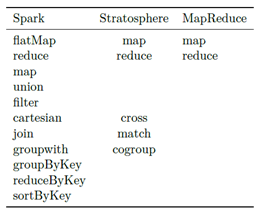
\includegraphics[width=0.5\textwidth]{Figures/batch_comparison.png}
\caption{Operators comparison}\label{fig-batch-comparison}
\end{figure}

In brief, MapReduce, Stratosphere and Spark have some common features: load balancing, and fault tolerance. Stratosphere extends MapReduce, offering further operations as shown in Fig. 2. Spark provides the in-memory processing mechanism and supports the interactive analyses. On the other hand Stratosphere offers optimisation mechanisms.

\subsection{Serving Layer} \label{subsec-lr-servinglayer}

\subsubsection{Introduction} \label{subsubsec-lr-servinglayer-intro}
Batch processing jobs are expected to run for hours, weeks, months or even years, which is not ideal for monitoring a data- infrastructure such as WLCG. Therefore, a serving layer is required for ad-hoc interactive queries. A few well known intensive Internet giants have developed tools to resolve this issue, which will be reviewed in the following section.

\subsubsection{Apache Drill} \label{subsubsec-lr-servinglayer-drill}
Apache Drill is a distributed execution engine that facilitates interactive, ad-hoc querying heterogeneous data sources on a large scale, which was inspired by Google's Dremel (7, 8). Its design goal is to scale to 10,000 servers or more and to process petabytes of data and trillions of records in seconds (8). As shown in Fig. 4, Drill’s architecture is made up of four components: query languages, which is responsible for parsing the user’s query and constructing an execution plan; a low-latency distributed execution engine that provides the scalability and fault tolerance needed to efficiently query petabytes of data; nested data formats, which are responsible for supporting various data formats (8). The initial goal is to support the column-based format used by Dremel (8). Finally, scalable data sources are responsible for supporting a variety of data sources. The initial focus is to leverage Hadoop as a data source (8).

\begin{figure}[H]
\centering
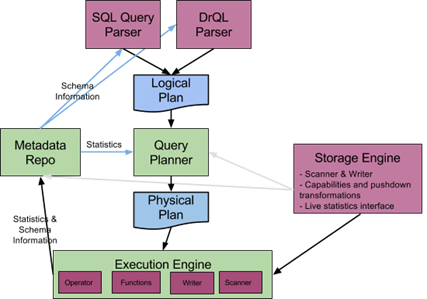
\includegraphics[width=0.5\textwidth]{Figures/drill.png}
\caption{Apache Drill Architecture}\label{fig-serving-drill}
\end{figure}

From a distribution perspective, Drillbits, each node’s instance of Drill, uses local memory and data. Queries can be made from any such instance (8). The co-ordination, query planning and optimisation, scheduling, and execution are then distributed.

\subsubsection{Cloudera Impala} \label{subsubsec-lr-servinglayer-impala}
Cloudera Impala is a massively parallel processing (MPP) architecture for performing SQL-like queries on HDFS and HBase storage as shown in Fig. 4, which does not employ the MapReduce model as other alternatives such as Hive (9). It leverages techniques such as columnar storage for performing really fast scans in the order of seconds of huge amounts of data in memory. All data in HDFS or HBase do not require Extraction, Transformation and Loading (ETL) so can be queried directly without any data movement or predefined schemas using SQL-like commands. Impala inherits inbuilt Hadoop security by integrating with Kerberos for authentication and role-based authorisation (9).

\begin{figure}[H]
\centering
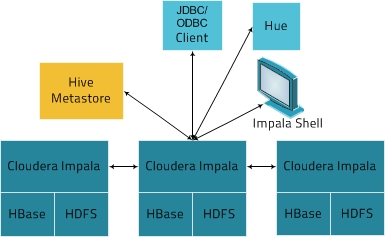
\includegraphics[width=0.5\textwidth]{Figures/impala.png}
\caption{Cloudera Impala}\label{fig-serving-impala}
\end{figure}

\subsubsection{Facebook’s Presto} \label{subsubsec-lr-servinglayer-presto}
Presto is a distributed low-latency, interactive and SQL-compliant query engine optimised for ad-hoc analysis (10). It also supports the majority of ANSI SQL subgroups, including complex queries, aggregations, joins, and window functions (10). All processing is carried out in-memory and pipelined across the network between steps, which should reduce the read/write to disk thus improving performance. The shortcomings of the system are its inability to write output data back to tables as it only supports the read-only mode. In Presto architecture as shown in Fig. 5, there is a coordinator that receives SQL queries from the client, which it then analyses, parses and then plans the execution (10). Then the scheduler connects the execution pipeline and assigns the jobs to worker nodes that reside closer to the data (10). The client then fetches the results.

\begin{figure}[H]
\centering
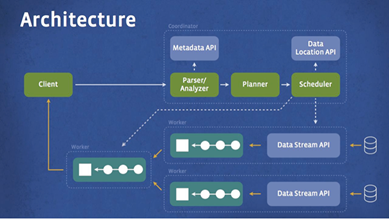
\includegraphics[width=0.5\textwidth]{Figures/presto.png}
\caption{Presto Architecture}\label{fig-serving-presto}
\end{figure}

The Presto framework is extendable so any storage can be plugged in; however, it require a connector that provides Presto with metadata, information on which nodes hold the data, and a way to actually fetch the data as a stream. The current version provides plugins for the following storage system: HDFS, Hive, HBase and Scribe (10).

\subsubsection{Apache Shark} \label{subsubsec-lr-servinglayer-shark}
Shark is a large-scale distributed and fault-tolerant, in-memory analytics system designed to be compatible with Hadoop (11, 12). In particular, Shark is fully compatible with Hive and supports HiveQL, Hive data formats, user-defined functions, HDFS, HBase and Amazon S3 (11). Shark provides the users with a mechanism to store or load their working set of data into custom columnar in-memory store and compresses them in order to reduce the storage space and execution time. Shark is a component that sits on top of Spark as shown in Fig. 6, which was discussed in the previous section. It also supports advanced techniques such as data co-partitioning and incorporation of machine learning into the workflow (12). Shark architecture contains an optimiser engine called partial DAG execution, which uses historical data information to dynamically adjust query and execution plans (12).

\begin{figure}[H]
\centering
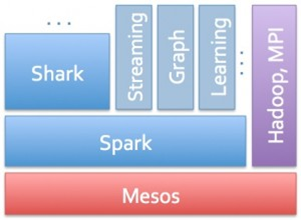
\includegraphics[width=0.5\textwidth]{Figures/shark.png}
\caption{Spark stack}\label{fig-serving-shark}
\end{figure}

\subsubsection{Comparison} \label{subsubsec-lr-servinglayer-comparison}
Hadoop was never built for real-time interactive ad-hoc querying; it mainly focuses on offline batch processing. This has resulted in a need for a new stack of technologies that could resolve high latencies. In recent years a few tools have emerged to address this issue, which have been listed in a previous section. In brief, Drill, Impala, Presto and Shark were developed to take advantage of in-memory temporary data locality. Spark and Drill support long-running queries and ad-hoc queries, whereas Impala and Presto do not support long running queries.

No fault-tolerance is implemented in Impala or Presto; when a node fails at the execution time then the queries need to be re-executed. However, Shark utilises an underlying Spark engine for fault-tolerance by exercising the lineage method, which is a technique used to recover missing pieces of RDDs by re-computing or rebuilding from the row data source (12). Impala and Shark were designed to take advantage of the existing Hive infrastructure, which uses the same metadata. In contrast, Drill and Presto were developed to provide distributed query abilities across various data stores. However, the current framework only supports Hadoop. Some of the published benchmarks state that Shark performs much better than Impala and Presto (13). However, there aren’t any benchmarks to compare it with Drill due to the fact that it is still under development. Shark provides a mechanism to utilise complex machine learning to embed with the analytics dataflow; however, Drill, Presto and Impala do not support this.

\subsection{Real-Time Layer} \label{subsec-lr-servinglayer}

\subsubsection{Introduction} \label{subsubsec-lr-reallayer-intro}
A speed layer is required to perform real-time analytics on fresh data as they are received. This is required to monitor the infrastructure proactively and trigger actions so the operation will run smoothly.

\subsubsection{Apache Storm} \label{subsubsec-lr-reallayer-storm}
Apache Storm is a distributed, real-time processing of unbounded streams of the data system (14). It is considered as an alternative to high-latency batch processing for processing data in low-latency near real-time. Storm can be embedded with the queuing and database technologies. It facilitates scalability by enabling users to determine how many worker nodes are required to execute a job and the number of parallelism (threads) on the topology configuration. It also uses an independent Apache technology called Zookeeper for coordinating the cluster, which also supports a cluster scale (14). The architecture employs a master-slave model (14). The master node has a daemon called Nimbus, which is responsible for distributing user applications to worker nodes, allocating jobs to the worker queue and monitoring the status of the worker nodes, which on failure will restart the node or reassign the task to other nodes (14). The slave nodes have a daemon called supervisor, which is accountable for checking the queue for new jobs (14). 

\begin{figure}[H]
\centering
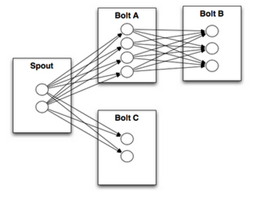
\includegraphics[width=0.5\textwidth]{Figures/storm.png}
\caption{Storm topology}\label{fig-real-storm}
\end{figure}

Storm uses tuples as its data model, which consists of a list of values. Groups of spouts and bolts are packaged into a topology, which is then deployed into clusters that will run infinitely, until killed manually. As shown in Fig. 7, the topology will consist of spouts, which are the source of streams; bolts, which consume the stream and process them; and stream grouping, which states how the data should flow (14). Storm also provides a tool called Distributed RPC, which enables developers to implement complex functions and execute them in Storm utilising parallelism.

\subsubsection{Simple Scalable Streaming System (S4)} \label{subsubsec-lr-reallayer-s4}
S4 is a distributed general-purpose platform that processes continuous unbounded streams of data (15). S4 employs the MapReduce and Actor programming models (15). Therefore, S4 utilises concurrent, decentralised and symmetric architecture, with each node sharing the same functionality and responsibility, which is imposed by utilising Apache ZooKeeper in order to coordinate the cluster. There aren’t any special nodes with special functions. The S4 model facilitates high availability and scalability on commodity hardware, low-latency by utilising local memory, fault-tolerance by check-pointing and summoning the standby server to take over the failed server tasks, and a pluggable framework so that it's more generic and new components can be plugged in (15).

\begin{figure}[H]
\centering
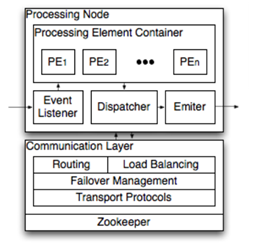
\includegraphics[width=0.5\textwidth]{Figures/s4.png}
\caption{S4 Architecture}\label{fig-real-s4}
\end{figure}

As shown in Fig. 8 processing nodes are the logical clusters of Processing Elements (PE), an entity that performs computation and transmits messages between PEs by using data events. The processing nodes are responsible for listening to events, executing functions on the incoming events, transmitting events and emitting output events. An event listener in the PN passes incoming events to the processing element container, which invokes the correct PEs corresponding to the unique key or generates a new instances of PEs (15). An application can be defined in terms of PEs with simple processing logic, and the framework instantiates one PE for each unique key in the stream. The communication layer provides load balancing, failover management and transport management (15). There are numerous special PEs that are available for performing tasks such as: count, aggregate, join and so forth (15).

\subsubsection{Amazon Kinesis} \label{subsubsec-lr-reallayer-kinesis}
Amazon Kinesis is a cloud-based service for real-time processing of high-volume stream data (16). Just as with any cloud service the Kinesis service is based on a metering system, which means you pay for the amount of throughputs and HTTP PUTs transactions used (16). Kinesis is proficient at consuming any amount of data from any number of sources, scaling up and down as needed. The Kinesis client library supervises load balancing, coordination and error handling automatically, so the developer only needs to focus on processing the data as it becomes available.

\begin{figure}[H]
\centering
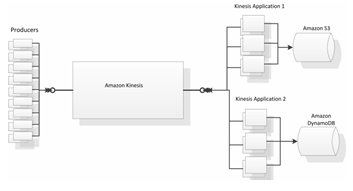
\includegraphics[width=0.5\textwidth]{Figures/kinesis.png}
\caption{Kinesis Architecture}\label{fig-real-kinesis}
\end{figure}

As shown in Fig. 9, Kinesis expects two components, which are the producer and worker (16). The producer accepts data from a source and converts them into a Kinesis stream, which is partitioned into 50KB data segments, then transferred into stream using HTTP PUTs methods (16). The worker then takes the data from the Kinesis stream and processes them. For scalability, the user has to take care of two things; adding or removing shards, depending on the required throughput capacity, and using the Kinesis client library and deploying the application into EC2 instance with the auto-scaling group.

\subsubsection{Apache Samza} \label{subsubsec-lr-reallayer-samza}
This is a distributed stream processing pluggable framework to run continuous computation on infinite streams of data (17). It’s designed to sit on top of the Kafka messaging queue for stream processing. It also utilises Apache Yet Another Resource Negotiator (YARN) for resource management and execution, which is responsible for deploying tasks in a distributed clusters, stream processor locality, co-partitioning of streams and providing security (17). The Samza framework is similar to batch processing as shown in Fig. 10.

\begin{figure}[H]
\centering
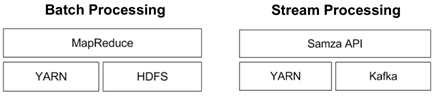
\includegraphics[width=0.5\textwidth]{Figures/samza.png}
\caption{Samza Architecture}\label{fig-real-samza}
\end{figure}

Samza partitions the message, assigns the partition key and sequence ID, and orders them in strict sequence. All messages matching the partition key would go to that partition.

It also facilitates a replayable mechanism so that a message can be reread when required. The stream processing is done by Samaza Job, which performs logical transformation on a set of input and emits outputs (17). Fault tolerances are managed by check-pointing, which enables failure recovery, and state management. This maintains the state of the intermediate data that need to be passed between processing; this is kept in the local disk with each task (17).

\subsubsection{Spark Streaming} \label{subsubsec-lr-reallayer-spark}
Spark Streaming is an extension of Spark that supports continuous processing (18, 19). As shown in Fig. 11, Spark Streaming is inspired by a batch system, such as dividing processing into sufficient sets so  that they can be replayed, assigning failed tasks to other nodes and decreasing batch sizes to tackle low latency (18).

\begin{figure}[H]
\centering
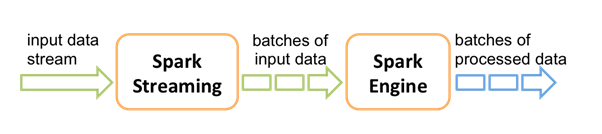
\includegraphics[width=0.5\textwidth]{Figures/spark_stream.png}
\caption{Spark Streaming data flow}\label{fig-real-spark}
\end{figure}
Spark Streaming provides two types of operators for building stream applications: transformation operators, which produce a new DStream from one or more parent streams, and output operators, which let the program write data to external systems (18). Spark Streaming supports all operators that are supported in Spark such as: Map, Reduce, GroupBy, Join and so forth. It also provides a mechanism to aggregate within a given window of time. It also allows the developer to apply Spark’s in-built machine learning algorithms, and graph processing algorithms on data streams (19). It supports checking pointing and fault tolerance, which it inherits from Spark.

\subsubsection{Comparison} \label{subsubsec-lr-reallayer-comparison}
The existing large-scale MapReduce data-processing platforms are highly optimised for batch processing, which typically operates on static data. Therefore, a paradigm was required to process data in real-time so business critical decisions can be made on time. This is where the evolution of the stream processing technologies listed above evolved.  

Storm, S4, Samza, Spark Streaming and Amazon Kinesis share the same aim, which is to provide a distributed, scalable and fault-tolerance infrastructure for processing continuous streams of data. Storm, Kineses, Samza and S4 are fundamentally like a pipeline where the source pushes discrete messages, which are then processed a record at a time. On the other hand, Spark Streaming follows a batch processing model where messages are collected and then processed at short-time intervals in a batch manner. However, this is prone to seconds-latencies compared with former technologies. Nevertheless, Spark does not replicate messages or checkpoints as a mechanism for fault-tolerance as with the other systems, which are liable to high disk I/O, network bandwidth usage and overheads of the operations itself. Spark utilises in-memory storage abstraction (RDD), which tracks the lineage steps used to build it, so in the event of failures, it can recompute the lost data using the cached steps. Storm does not support managing states, whereas S4, SAMZA and Kinesis provide tools to manage them locally or remotely. Storm is user-oriented, as it gives full control to the developers on how it should be configured so an external database can be used to store the states; however, this is costly, in terms of performance. Nevertheless, Samza provides a much better mechanism to minimise remote communication by keeping the state located locally with the tasks and only when a state is modified, will it invoke a remote method for an update. To the best of knowledge all the stream platforms discussed above utilise an in-memory mechanism for processing, except for Amazon Kinesis. Although in-memory processing accelerates low-latencies, this could raise a new issue in terms of flushing out the memory, in particular for S4. A complex application in utilising the S4 framework will generate a large number of unique processing elements as it has been designed to do so, which will occupy a large portion of the memory and could degrade performance. However, there is a mechanism called Time-to-Live that explicitly configures how long the PE should live without any event communication before the memory is reclaimed, but this will result in loss of the state of the PE. However, there is a method to overcome this issue by applying priority or importance of the PE object, which will be customised to the developer.

\subsection{Summary} \label{subsec-lr-tech-summ}
In the previous section, a brief overview of the different technology that supports batch processing, interactive ad-hoc queries and real-time analytics is reviewed. Most of the technology was developed by companies concentrating on their use cases. For some, performance is important, whereas for others fault-tolerance and recovery are important, and only one can be achieved by trading-off the other. So it’s not practical to have a perfect technology tailored for one requirement. Therefore, it’s important to distinguish and prioritise what is essential for the desired system and what can be compromised. 

When you have separate technologies for each layer such as batch/ serving / speed layers, it will become very difficult and complex to maintain the infrastructure. Hence, it will be interesting to explore the Spark stack as it supports batch processing, ad-hoc querying and stream processing. It uses the same processing model and data structures for batch processing and Spark Streaming, which enables ad-hoc queries on streams and combines streams with historical data using the same high-level APIs. Therefore, it simplifies development, deployment and maintenance as the codes can be reused between layers.



%\addcontentsline{toc}{chapter}{Experimentation and Evaluation}
\chapter{An efficient strategy for the collection and storage of petabytes of data for computation} \label{data-pipe}

%\section{Motivations} \label{Motivations}

\section{Abstract} \label{pipe-abstract}
In recent years, there has been an increasing amount of data being produced and stored, which is known as Big Data. The social networks, internet of things, scientific experiments and commercial services play a significant role in generating a vast amount of data. Three main factors are important in Big Data; Volume, Velocity and Variety. One needs to consider all three factors when designing a platform to support Big Data. A scientific experiment such as the Large Hadron Collider (LHC) is a data-intensive experiment, which is estimated to produce a volume of about 30 petabytes of data, annually. The velocity of these data that are propagated will be extremely fast. Traditional methods of collecting, storing and analysing data have become insufficient in managing the rapidly growing volume of data. Therefore, it is essential to have an efficient strategy to capture these data as they are produced. In this paper, a number of models are explored to understand what is the best approach for collecting and storing Big Data for analytics. Also, performance measurement of full execution cycles of these approaches on the monitoring of the Worldwide LHC Computing Grid (WLCG) infrastructure for collecting, storing and analysing is presented. Moreover, the models discussed are applied to a community driven software solution, Apache Flume, to show how they can be integrated, seamlessly.


%\linenumbers

\section{Introduction} \label{lbl-intro}
The field of data science has become a widly discussed topic in recent years due to a data explosion, especially with scientific experiments such as the Large Hadron Collider (LHC) at CERN and commercial businesses keen to enhance their competitiveness by learning about their customers to provide tailor made products and services, dramatically increasing the usage of sensor devices. The challenge of handling big volumes of data has been taken on by many companies, particularly those in the Internet domain, leading to a full paradigm shift in methods of data archiving, processing and visualisation. A number of new technologies have appeared, each one targeting specific aspects of big-scale distributed data-processing. All these technologies, such as batch computation systems (e.g. Hadoop) and non-structured databases (e.g MongoDB), can handle very large data volumes with little finacial cost. Hence, it becomes necessary to have a good understanding of the currently available technologies to develop a framework which can support efficient data collection, storage and analytics.

The core objectives of the presented study were the following:
\begin{itemize}
  \item Propose and design efficient approaches for collecting and storing data for analytics that can also be integrated with other data pipelines seamlessly.
  \item Implement and test the performance of the approaches to evaluate their design.
\end{itemize}

\section{Background} \label{lbl-review}
Over the past several years there has been a tremendous increase in the amount of data being transferred between Internet users. Escalating usage of streaming multimedia and other Internet based applications has contributed to this surge in data transmissions. Another facet of the increase is due to the expansion of Big Data, which refers to data sets that are many orders of magnitude larger than the standard files transmitted via the Internet. Big Data can range in size from hundreds of gigabytes to petabytes \cite{Verki1}.

Within the past decade, everything from banking transactions to medical history has migrated to digital storage. This change from physical documents to digital files has necessitated the creation of large data sets and consequently the transfer of large amounts of data. There is no sign that the continued increase in the amount of data being stored and transmitted by users is slowing down. Every year average Internet users are moving more and more data through their Internet connections. With the growth of Internet based applications, cloud computing, and data mining, the amount of data being stored in distributed systems around the world is growing rapidly. Depending on the bandwidth of these connections and the size of the data sets being transmitted, the duration of transfers could potentially be measured in days or even weeks. There exists a need for an efficient transfer technique that can move large amounts of data quickly and easily without impacting other users or applications \cite{Verki1}.

In addition to corporate and commercial data sets, academic data are also being produced in similarly large quantities \cite{Aamnitchi2}. To give an example of the size of the data sets utilised by some scientific research experiments, a recent study observed a particle physics experiment (DZero) taking place at the Fermi Lab research center. While observing the DZero experiment between January 2013 and May 2015, Aamnitchi et al. \cite{Aamnitchi2} analysed the data usage patterns of users. They found that 561 users processed more than 5 petabytes of data with 13 million file accesses to more than 1.3 million distinct data files. An individual file was requested by at most 45 different users during the entire analysed time period (2013 to 2015).

In the DZero experiment, and many like it, scientists are generating datasets with an extremely large number of data files. Use of entire datasets is quite popular amongst users, however the individual data files in these sets are rarely used concurrently since they are so numerous.

There are many scientific research initiatives that have similar data demands. The most popular example today is the LHC. This experiment is well known and thousands of researchers in the physics and computer science fields are involved. The four experiments being conducted at the LHC generate petabytes of data annually \cite{Minoli3, Nicholson4}. One experiment, ALICE, can generate data at the rate of 1.25 GB/s. Figure \ref{fig:lhc_data} illustrates the growth in the size of data sets being created and stored by CERN. This graph shows the total amount of storage (both disk and tape) utilised by all of the top-level servers in the CERN organisation. The amount of data stored in the system has grown at a steady pace over the past 3 years and is expected to grow faster now that the intensity of their experiments is increasing, which will result in more data collected per second \cite{LHC5}. 

Geographically dispersed researchers eagerly await access to the newest datasets as they become available. The task of providing and maintaining fast and efficient data access to these users is a major undertaking. Also, monitoring computing behaviours in the Worldwide LHC Computing Grid (WLCG), such as data transfer, data access, and job processing is crucial for efficient resource allocation. This requires the gathering of metadata, describes the data (e.g. transfer time), from geographically distributed sources and the processing of such information to extract the relevant value for the WLCG group \cite{Magnoni20}. Since the CERN experiments are so well known and many studies have been conducted on their demands and requirements, one can use the CERN LHC experiments as a suitable case study for this research.

To meet the computing demands of experiments like those at the LHC, a specialised distributed computing environment is needed. Grid computing fits the needs of the LHC experiments and other similar research initiatives.

\begin{figure}[H]
  \centering
  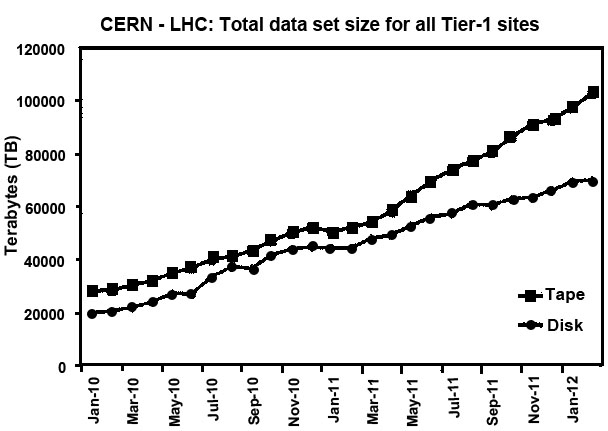
\includegraphics[width=100mm]{./Figures/lhc_data_size.jpg}
  \caption{\small Size of CERN LHC experimental data sets over the past years. The total disk and tape storage amounts aggregated for all Tier-1 locations in the CERN grid (adapted from \cite{LHC5}).}\label{fig:lhc_data}
\end{figure}

The Worldwide LHC Computing Grid (WLCG) was created by CERN in 2002 in order to facilitate the access and dissemination of experiment data. The goal of the WLCG is to develop, build, and maintain a distributed computing infrastructure for the storage and analysis of data from LHC experiments \cite{Knobloch6}. The WLCG is composed of over a hundred physical computing centers with more than 100,000 processors \cite{LHCGrid7}. Since the data sets produced by the LHC are extremely large and highly desired, the WLCG utilises replication to help meet the demands of users. Copies of raw, processed, and simulated data are made at several locations throughout the grid.

The WLCG utilises a four-tiered model for data dissemination. The original raw data is acquired and stored in the Tier-0 center at CERN. This data is then forwarded in a highly controlled fashion on dedicated network connections to all Tier-1 sites. There are eleven Tier-1 sites located in Canada, Germany, Spain, France, Italy, Nordic countries, Netherlands, Taipei, United Kingdom and USA.

The role of the Tier-1 sites varies according to the particular experiment, but in general they have the main responsibility for managing the permanent data storage - raw, simulated, and processed data - and providing computational capacity for processing and analysis \cite{Knobloch6}. The Tier-1 centers are connected with CERN through dedicated links (Figure \ref{fig:lhc_network}) to ensure high reliability and high-bandwidth data exchange, but they are also connected to many research networks and to the Internet \cite{LHCGrid7}. The underlying components of a Tier-1 site consist of online (disk) storage, archival (tape) storage, computing (process farms), and structured information (database) storage. Tier-1 sites are independently managed and have pledged specific levels of service to CERN. It is therefore left to the site’s administrators to guarantee that these services are reliably provided.

The Tier-2 sites are used for Monte Carlo event simulation and for end-user analysis. Any data generated at Tier-2 sites is forwarded back to Tier-1 centers for archival storage.

Other computing facilities in universities and laboratories are able to retrieve data from Tier-2 sites for personal processing and analysis. These sites constitute the Tier-3 centers, which are outside the scope of the controlled WLCG project and are individually maintained and governed. Tier-3 sites allow researchers to retrieve, host, and analyse specific datasets of interest. Freed from the reprocessing and simulation responsibilities of Tier-1 and Tier-2 centers, these Tier-3 sites can devote their resources to their own desired analyses and are allowed more flexibility with fewer constraints \cite{Grim8}. As there are thousands of researchers eagerly waiting for new data to analyse, many users will find less competition for time and resources at Tier-3 sites than at the Tier-2 sites.

It is important to note that users connecting to either Tier-2 or Tier-3 sites will use public, shared network connections, including the Internet. Grid traffic and normal World Wide Web traffic will both be present on these shared links. A user will also be sharing the site that they access with multiple other users. These factors can affect the performance of the data transfer between the selected retrieval site and the user. Retrieving these large data files also places a burden on shared resources and impacts other grid and non-grid users. When it comes to retrieving data in the WLCG, a normal user (depending on their security credentials) can access data on either Tier-2 and Tier-3 sites. The user would select a desired site and issue a request for a specific data file. Selecting a site to utilise can be a complicated task, with the performance a user obtains being dependent on the location chosen.

\begin{figure}[H]
  \centering
  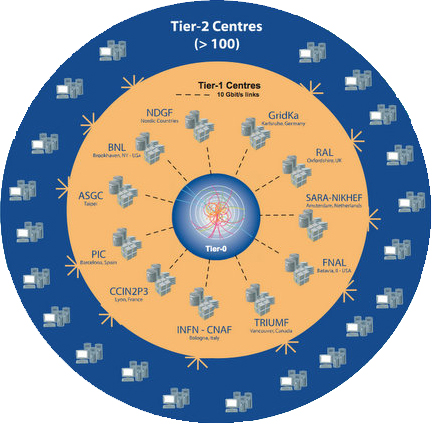
\includegraphics[width=100mm]{./Figures/lch_network.jpg}
  \caption{\small WLCG Tier-1 and Tier-2 connections \cite{LHCGrid7}.}\label{fig:lhc_network}
\end{figure}

Grid computing has emerged as a framework for aggregating geographically distributed, heterogeneous resources that enables secure and unified access to computing, storage and networking resources \cite{Foster9} for Big Data. Grid applications have vast datasets and/or complex computations that require secure resource sharing among geographically distributed systems. The term “grid” was inspired by the electrical grid system, where a user can plug in an appliance to a universal socket and have instant access to power without knowing exactly where that power was generated or how it came to reach the socket \cite{Foster9}.

The vision for grid computing was similar. A user could simply access as much computing power as required through a common interface without concern for who was providing the resources. Currently, grids have not yet reached that level of simplicity.

Grids offer coordinated resource sharing and problem solving in dynamic, multi-institutional virtual organisations \cite{Foster10}. A virtual organisation (VO) comprises a set of individuals and/or institutions having access to computers, software, data, and other resources for collaborative problem-solving or other purposes \cite{Laure11}. A grid can also be defined as a system that coordinates resources that are not subject to centralised control, using standard, open, general-purpose protocols and interfaces in order to deliver nontrivial qualities of service \cite{Foster12}. However, a number of new technologies have emerged for handling big-scale distributed data-processing, for example Hadoop, where the belief is that moving computation to where data reside is less time consuming than moving data to a different location for computation when dealing with Big Data. This is certainly true when the volume of data is very large because this approach will reduce network congestion and improve the overall performance of the system. However, a key grid principle contradicts with this as computing elements (CE) and storage elements (SE) in this scheme should be isolated. Currently, a lot of scientific experiments are beginning to adopt the ``new" Big Data technologies, in particular for metadata analytics at the LHC, hence the reason for the presented study.

Parallelising is used in order to enhance computations of Big Data. The well known MapReduce \cite{Dean13} framework that has been used in this paper has been well developed in the area of Big Data science and has the parallelisation feature. Its other features are its inherent data management and fault tolerant capabilities.

The Hadoop framework has also been employed in this paper. It is an open-source MapReduce software framework. For its functions it relies on the Hadoop Distributed File System (HDFS) \cite{Shvachko14}, which is a derivative of the Google File System (GFS) \cite{Ghemawat15}. In its function as a fault-tolerance and data management system, as the user provides data to the framework, the HDFS system splits and replicates input on some cluster nodes.

	The approaches for collecting and storing Big Data for analytics are applied on a community-driven software solution such as Apache Flume in this research in order to understand how it can be integrated seamlessly. Apache Flume is used for effectively gathering, aggregating, and transporting large amounts of data. It has a flexible and simple architecture, which makes it fault tolerant and robust with tunable and recovery mechanisms. It uses a simple extensible data model that allows online analytic applications \cite{Flume16}.

\section{Design and methodology} \label{lbl-dm}
When data messages are consumed from the transport layer and written into storage, there will most likely be some sort of data transformation carried out before storage in the storage layer. Such a transformation could be extracting the body from the message and removing the header as it is not required, or serialisation or compression. There needs to be a strategy in place to carry out the required transformation as this will play a significant role in improving the performance of subsequent computations. In this paper three different approaches were explored:

\begin{enumerate}
	\item Implement the data transformation logic within the data pipeline. Therefore, the messages, M, will be read by the consumer, to apply the transformation \(\langle\circlearrowright T\rangle \) and to write the results into the storage layer, S, for analytics \( \langle\circlearrowright A\rangle \):
	
		\centerline{\(M \xrightarrow[]{\langle\circlearrowright T\rangle}S\rightarrow  \langle\circlearrowright A\rangle \)}
		
	\item Write the raw messages, M, directly into storage layer, S, without any modification. Then there is another intermediate job \(\langle\circlearrowright iT\rangle\) that reads the raw data from storage, transforms the data and writes the results into a new path but to the same storage layer for analytics \( \langle\circlearrowright A\rangle \):
	
	\centerline{\(M\rightarrow S\xrightarrow {\langle\circlearrowright iT\rangle} S\rightarrow   \langle\circlearrowright A\rangle \)}
	
	\item Write the raw messages, M, into the storage layer, S, without any modification. Let the analytics \( \langle\circlearrowright A\rangle \) jobs carry out the transformation \(\langle\circlearrowright T\rangle \):
	
	\centerline{\(M \rightarrow S\rightarrow   \langle \langle\circlearrowright T\rangle +\langle\circlearrowright A\rangle \rangle \)}
	
\end{enumerate}

The first approach is the traditional way of transforming data. However, this relys too much on the data pipeline. If the data pipeline is replaced then the transformation logic would need to be reimplemented. Therefore, it is an inefficient design.

The second approach has two benefits as the transformation logic is moved to a centralised location and untampered raw data are stored as well as the transformed data. Therefore, in any case of inconsistency with the transformed data, it can be reconstructed from the raw data. This is not possible with the first method becasuse as soon as the data are transformed the raw data are discarded. Nevertheless, the second approach is very complex as there is a requirement for a job to transform the data and it raises the question of when and how this job should be scheduled. This approach also requires increased data storage as both raw and transformed data will be kept. A transformation job could be used here to compress the raw data and archive it to reduce the amount of storage required.

The third option is very simple and straight forward, as the raw data will be written into the storage layer without any modification. The transformation will only take place at the data analytics time. The transformation logic can be implemented in a shared library, which can be imported into any analytics jobs. Therefore, the transformation will take place as and when it is required. This way, the untempered raw data is still kept in the storage layer and no additional job or storage is needed for data transformation. Nonetheless, this method does add an extra execution time overhead to the analytics jobs and repetition of transformation. This should, however, not be too much of a problem as Big Data technologies are built to enhance computation speed by parallelising jobs. Hence, this arrangement should not significantly affect the execution time.

\subsection{Implementation} \label{lbl-implementation}
	The data pipeline presented in this paper uses Dirq library that offers a queue system using the underlying filesystem for storage for consuming messages, which allows concurrent read and write operations \cite{Dirg17}. Therefore, it can support a variety of heterogeneous applications and services that can write messages and have multiple readers reading the messages. The data pipeline was developed using the Hadoop native library that reads messages from the Dirq and writes them into HDFS using an appending mechanism. The Hadoop software framework was originally designed as create-once-read-many times system \cite{Hadoop18}. Therefore, appending was not available in the initial software release but later versions, 2.0 onwards, supported this mechanisum. Hadoop also has the benefit of working well with a few large files but is not so efficient when working with a large number of small files. The appending method is convenient as it allows for the creation of a single large file.

For the first approach, the data will be consumed from the Dirq, transformed and written into HDFS. The implementation of the second approach is similar to the first one with exception of no transformation. However, it requires chained MapReduce jobs in a centralised Hadoop cluster in order to take the raw data that has not previously been processed, and apply the appropriate data transformation, merge the transformed data with previously transformed data, delete the old transformed data, update the raw data as processed and merge and compress the raw data. An issue was encountered during testing of this appproach where it was found that data that were not processed by the transformation job were not available for analytics. The third approach is again like the second approach in that no transformation is carried out in the data pipeline, but the transformation logic is implemented in a common library and is available to be imported into any analytics jobs. Therefore, the transformation can be carried out as and when it is required. This approach will not have the issue of data unavailability as present in the other approaches as all written data will be picked up by the analytics jobs and the transformation will be done as and when required. All three approaches were implemented as a daemon that continuously ran on the CERN test infrastructure but will only check for data every 5 minutes, which causes a delay in making the data available for the analytics jobs.

In order to decrease the data aggregation delay from the data pipeline and to evaluate how easy it is to migrate to a different data pipeline, Apache Flume was used. Apache Flume is a community-driven software solution that receives messages from the transport layer and writes them into HDFS. There are three ways to flush consumed data into HDFS: periodically based on the elapsed time, the size of data or the number of events \cite{Flume16}. As expected, the first approach was complex as all the transformation logics were in the custom data pipeline so the transformation logics had to be reimplemented into Apache Flume. The second and third approach made the migration extremely simple, as all the transformation logics were implemented within the storage layer. But, as noted before, the second approach adds complexity to the storage layer, as it requires a chain of actions for data transformation. The third approach was the far simpler one, as no transformation was done at the Apache Flume side and no complexity of transformation was added at the storage layer. However, all three approaches encountered a common problem when Apache Flume pushes the events but does not flush the file until the configured file roll time is met, e.g. every 1 hour, the data being unavailable for computation during this time. While HDFS supports appending functionality, and the custom data pipeline, Apache Flume does not support it. The analytics jobs were able to read the data that were written by the custom data pipeline but not those written by Apache Flume. Therefore, the appending functionality was stripped out from the custom pipeline and implemented into Apache Flume, making it a custom library (see Algorithm~\ref{alg:append_alg}). With this amendment, Apache Flume was able to write a single file and append it while analytics jobs were able to read the data while the data were being written into HDFS.



\makeatletter
\def\BState{\State\hskip-\ALG@thistlm}
\makeatother


\begin{algorithm}[H]
\caption{File appending algorithm for Apache Flume: adding a close and reopen at every push to get the append behavior.}\label{alg:append_alg}
\begin{algorithmic}[1]
\Procedure{create-global-data-file-writer}{}
\State $ \text{declare a global DataFileWriter object}$
\State $ \text{create a file in HDFS}$
\State $ \text{initialise the file to global DataFileWriter}$
\item[]
\EndProcedure
\end{algorithmic}
\begin{algorithmic}[1]
\Procedure{consume-messages-and-sync-flush}{}
\State $ \text{create a temp  DataFileWriter refelecting(reopen) the global DataFileWriter}$
\State $ \text{consume all messages}$
\State $ \text{append mesages using temp DataFileWriter}$
\State $ \text{close temp DataFileWriter WHEN messages \( <=0 \)}$
\item[]
\EndProcedure
\end{algorithmic}
\begin{algorithmic}[1]
\Procedure{roll-files}{}
\State $ \text{close the global DataFileWriter} $
\item[]
\EndProcedure
\end{algorithmic}
\end{algorithm}


\section{Results and discussion} \label{lbl-results}
The three implementations discussed for this study were evaluated on the WLCG infrastructure that provides the computing resources to store, distribute and analyse the 30 petabytes of data, annually generated by the LHC and distributed around 150 computing centres around the world \cite{Gardner19}. LHC experiments utilise the XRootD protocol for data transfers and data access \cite{Gardner19}. This protocol is heavily used, hence the propagation of log messages is very intensive.

It is very complicated to carry out performance measurements on the three approaches, as they deploy different methods for consuming, writing and transforming the data. Therefore, in order to get a meaningful performance measurement, a full computation cycle was carried out; including consuming messages, writing to HDFS and carrying out a simple analytics job on those data. The full cycle was broken into three segments:

\begin{enumerate}[1.]
\item Data ingestion with data transformation and without data transformation.
\item Intermediate data transformation using a MapReduce job.
\item A simple statistical analytic computation using a MapReduce job with and without data transformation.
\end{enumerate}

In order to evaluate the proposed models, it was decided to push messages from the broker in batch sizes ranging from 10k to 100k. Data ingestion and analytics were conducted a few times for each batch of messages in order to capture an average performance time. The performance measurements were carried out on a heterogeneous Hadoop cluster that consisted of 15 nodes (8 nodes: 32 cores/64 GB, 7 nodes: 4 cores/8 GB).


\subsection{Performance results of data ingestion with and without data transformation} \label{lbl-perf-dpipe}
The first approach had to consume all messages from Dirq, apply a simple data transformation, which involved taking the source and destination IP address from the message and using a topology mapping file to determine the domain address and replace the IP address with the domain, and finally converting the data file into Avro format, which is a data serialisation framework that serialises the data into a compact binary format and writes the file into HDFS. As shown in Figure \ref{fig:pipe}, this approach (pre-trans-avro) is slower than the second approach (raw-json), which just reads the raw messages in JavaScript Object Notation (JSON), an easy-to-read format, and writes them into HDFS. The second approach is the fastest compared with the first and third approaches (raw-avro), which read raw data, convert them into Avro format and write them into HDFS. The third approach is faster then the first approach because it does not do any transformation.

\begin{figure}[H]
  \centering
  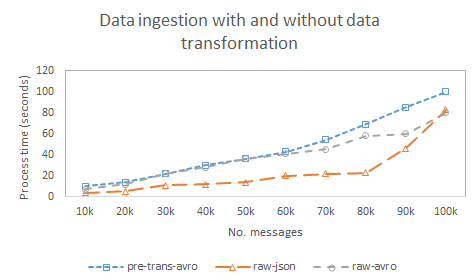
\includegraphics[width=100mm]{./Figures/datapipe_perf.jpg}
  \caption{\small Data ingestion from message queue to HDFS with and without data transformation.}\label{fig:pipe}
\end{figure}


Figure \ref{fig:ds} shows data representing unprocessed messages from the broker, raw JSON messages, a pre-transformed Avro and raw Avro file written into HDFS by the custom data pipeline. The Avro files are smaller than the JSON file and unprocessed data because they are serialised into binary format. However, the pre-transformed Avro file is larger than the raw Avro file because transformation was applied.

\begin{figure}[H]
  \centering
  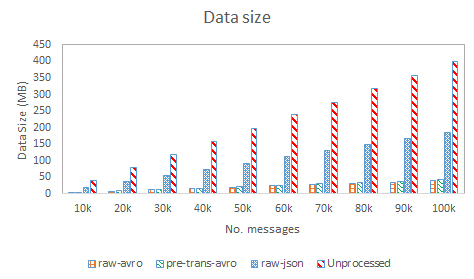
\includegraphics[width=100mm]{./Figures/data_size.jpg}
  \caption{\small Data size of the messages that were stored into HDFS with and without data transformation.}\label{fig:ds}
\end{figure}


\subsection{Performance results of intermediate data transformation using a MapReduce job} \label{lbl-perf-inter}
This test is designed to measure the performance of the intermediate transformation done on a centralised Hadoop cluster. As shown in Figure \ref{fig:mr_trans}, only the raw JSON data will go through this transformation, as the pre-transformed Avro file has already been transformed at the data pipeline level and the raw Avro data will be transformed at the analytic time when it is required. Transforming the data using an intermediate job is very expensive in terms of execution time, as they are chained MapReduce jobs that will transform, aggregate and merge the data. The majority of the overhead was used for finding resources and submitting the chained jobs to the Hadoop cluster.

\begin{figure}[H]
  \centering
  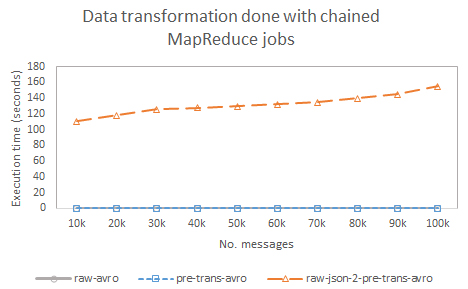
\includegraphics[width=100mm]{./Figures/mr_trans_perf.jpg}
  \caption{\small Intermediate MapReduce job for data transformation. Only the raw JSON messsages are transformed with the MapReduce job.}\label{fig:mr_trans}
\end{figure}

\subsection{Performance results of a simple analytic computation with and without data transformation} \label{lbl-perf-mr}
The final step of the evaluation cycle was to carry out a simple computation on the 100k messages dataset and measure the performance. Two sets of analytics jobs were implemented to compute a summary view of the XRootD operations, performed by the different users for each WLCG site belonging to the XRootD federation \cite{Gardner19}. An analytics job was modified to include the data transformation prior to the computation. The modified job was executed on the raw Avro data. As shown in Figure \ref{fig:mr_stats}, an extra overhead was added to the modified analytics job when compared with unmodified job that computed pre-transformed data, but the computation was seamless, as the MapReduce framework adopts a parallel programming model. Therefore, the jobs will be split into multiple tasks and will be sent to data nodes where the data reside.

\begin{figure}[H]
  \centering
  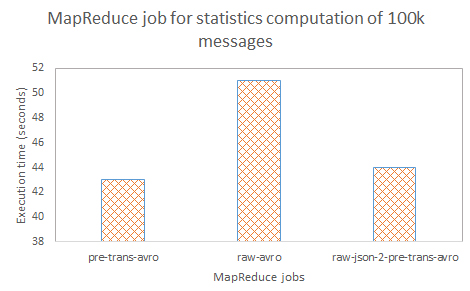
\includegraphics[width=100mm]{./Figures/mr_stats_perf.jpg}
  \caption{\small Performance measurements of the statistic computation were done on pre-transformed and the raw 100k dataset.}\label{fig:mr_stats}
\end{figure}

\subsection{Summary of the performance results} 
In order to understand which approach performed better, the execution time of the largest dataset of 100k messages was selected from Sections \ref{lbl-perf-dpipe}, \ref{lbl-perf-inter} and \ref{lbl-perf-mr} and the total is presented in Table \ref{table:tbresult}. It is clear that writing the raw Avro data into HDFS and letting the analytics do the transformation outperforms the other two approaches. The slowest seems to be the raw JSON file and having an intermediate job for transformation, which is understandable as they are chained jobs, which will add extra overheads. The pre-transformed Avro file by the data pipeline is not far from raw Avro data. But it will be beneficial to keep a copy of the untempered raw file in HDFS and let the analytics job do the transformation, which is better than pre-transformation as the authenticity is lost once the transformation is done and stored in HDFS.

\begin{table}[H]
\caption{Total sum of execution time for 100k dataset from Sections \ref{lbl-perf-dpipe} , \ref{lbl-perf-inter} and  \ref{lbl-perf-mr} are presented.}

\centering
    \begin{tabular}{ | l | l | l | l | l |}
    \hline 
 \multicolumn{1}{|p{2cm}|}{\centering \bfseries Transformation}
& \multicolumn{1}{|p{2cm}|}{\centering \bfseries Section \ref{lbl-perf-dpipe} \\ (secs)}
& \multicolumn{1}{|p{2cm}|}{\centering \bfseries Section \ref{lbl-perf-inter} \\ (secs)}
& \multicolumn{1}{|p{2cm}|}{\centering \bfseries Section \ref{lbl-perf-mr} \\ (sec)}
& \multicolumn{1}{|p{2cm}|}{\centering \bfseries Total \\ (secs)} \\\hline
    pre-trans-avro-mr & 100 & 0 & 43 & 143  \\ \hline
    raw-avro-mr & 80 & 0 & 51 & 131 \\ \hline
    raw-json-2-pre-trans-avro-mr & 83 & 155 & 44 & 282 \\ \hline
    \end{tabular}
		\label{table:tbresult}
\end{table}

%However, the is not much overhead to the data pipeline as it reads the messages and write the data into HDFS directly. Nevertheless, the data transformation and aggregation job is very expensive. In fact, it is extravagant than the first approach. %There is not additional overhead to data pipeline as same as the second approach but it does not have a separate complex job for data transformation. 



\subsection{Evaluation of Apache Flume} \label{lbl-flume}
There is still 5 minutes delay in polling data from the message queue. In order to eliminate the polling latency, the custom-made Apache Flume data collectors, as explained in \ref{lbl-implementation}, that utilise the appending mechanism were used. The performance test results shows that the third approach is optimal. Therefore, Apache Flume agents were configured to consume messages and flush them into HDFS directly. Figure \ref{fig:flum_stats} show spikes in the total number of messages propagated with a rate \( > \) 1 kHz, and it can be seen that Apache Flume seamlessly absorbs the load on its single virtual machine. Meanwhile, the old Oracle-based consumers used by WLCG, running on two production virtual machines, were struggling to keep up, causing a backlog of message stored in the broker.

\begin{figure}[H]
  \centering
  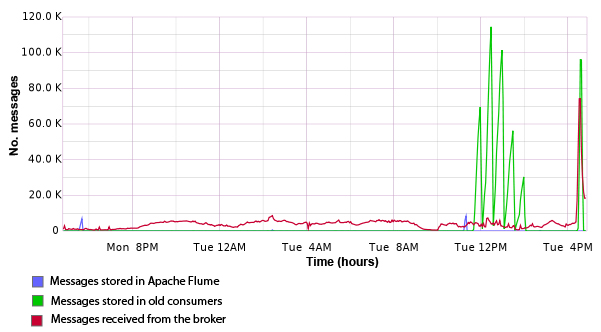
\includegraphics[width=100mm]{./Figures/flume_msg.jpg}
  \caption{\small Spikes of messages with a rate \( > \) 1 kHz. The red line is the messages received from the broker, green denotes the messages stored in old consumers, and blue denotes the messages stored in Apache Flume.}\label{fig:flum_stats}
\end{figure}


\section{Conclusion} \label{lbl-concl}
The approaches for consuming and storing data for analytics presented in this paper show how important it is to select the correct model for efficient performance and technology migration. It is clear from the study that keeping the main logic in a centralised location will simplify the technological and architectural migration. The performance test results show that eliminating any transformation at the data ingestion level and moving it to the analytics job is beneficial as the overall process time is reduced; untempered raw data are kept in the storage level for fault-tolerance, and the required transformation can be done with analytics jobs when required using a framework such as MapReduce. The WLCG group has adopted this approach, and it has been used for collecting, storing, and analysing metadata since April 2015 \cite{Magnoni20}. This approach can be easily applied to other use cases (e.g. business, for collecting customer interest datasets) and is not restricted to scientific applications.

%\section*{References}

%\bibliography{mybibfile}






%\addcontentsline{toc}{chapter}{Monitoring WLCG with lambda-architecture}
\chapter{Monitoring WLCG with lambda-architecture} \label{lambda-eva}

%\section{Motivations} \label{Motivations}

\section{The evolution of WLCG activities monitoring} \label{lambda-intro}

Monitoring computing activities in the Worldwide LHC Computing Grid (WLCG)
\cite{wlcg}, such as job processing, data access and transfers or sites
availability, requires the gathering of monitoring data from
geographically-distributed sources and the processing of such information to
extract the relevant value for WLCG users, computing teams of the WLCG
organizations and WLCG site operators.  Current monitoring systems have proven to be
a solid and reliable solution to support WLCG functions and operations during
LHC data-taking years.  A variety of data coming from different services and
experiment-specific frameworks is gathered, processed and archived and a
generic web-based dashboard provides a uniform and customisable monitoring
interface for scientists and sites. Nevertheless, the current architecture,
where relational database systems are used to store, to process and to serve
monitoring data, has limitations in coping with the foreseen increase in the
volume (e.g.  higher LHC luminosity) and the variety (e.g. new data-transfer
protocols and new resource-types, such as cloud-computing) of WLCG monitoring
events. This paper presents the new data store and analytics platform which is
going to be used for the evolution of WLCG activities monitoring.

\subsection{WLCG data activities dashboards} 

The Experiment Dashboard (ED) \cite{Andreeva2009} is a generic monitoring
framework which provides uniform and customisable web-based interfaces for
scientists and sites. Monitoring events, such as data transfers or data
processing jobs reports, are collected and analysed to produce summary
time-series plots used by operators and experts to evaluate WLCG computing
activities. The WLCG Data acTivities (WDT) dashboards are a set of monitoring
tools based on the ED framework which are used to monitor data access and
transfer across WLCG sites via different protocols and services. Monitored
services include the ATLAS Distributed Data Manamegement (DDM) system, XRootD
and HTTP federations and the File Transfer Service (FTS).  The WDT use case is
one of the most data intensive ED applications. Figure \ref{fig:wdt} presents
the daily volume of monitoring information handled by WDT, with an overall
average of more than 20 million daily monitoring events.  Today, WDT
dashboards are suffering from the limitation of the current processing
infrastructure, as presented in the next section. For this reason, WDT is taken
as a case study for the new analytics platform.

% In the next future,
%the WLCG monitoring infrastructure have to cope with an extension of the volume
%(e.g. higher LHC luminosity) and the variety (e.g. new data-transfer protocols
%and new resource-types, as cloud-computing) of the monitoring data. 

%The task requires a sound knowledge of distributed systems theory and concepts together with a deep understanding of the new technology stack for large-scale data analysis. The project will be done relying on facilities and experience f%rom the Agile Monitoring initiative of the CERN IT department.

%The Experiment Dashboard (ref) is a generic web-based dashboard framework which is used to provide uniform and customisable monitoring interface for scientists and sites. The Figure in \ref{fig:wdtv} shows the daily volume of monitoring information processed by the different dashboards. While being a solid a reliable monitoring solution, the foreseen increase in data volume and variety of monitoring requires an evolution of the current archive and processing technology.   

\begin{figure}
  \centering
  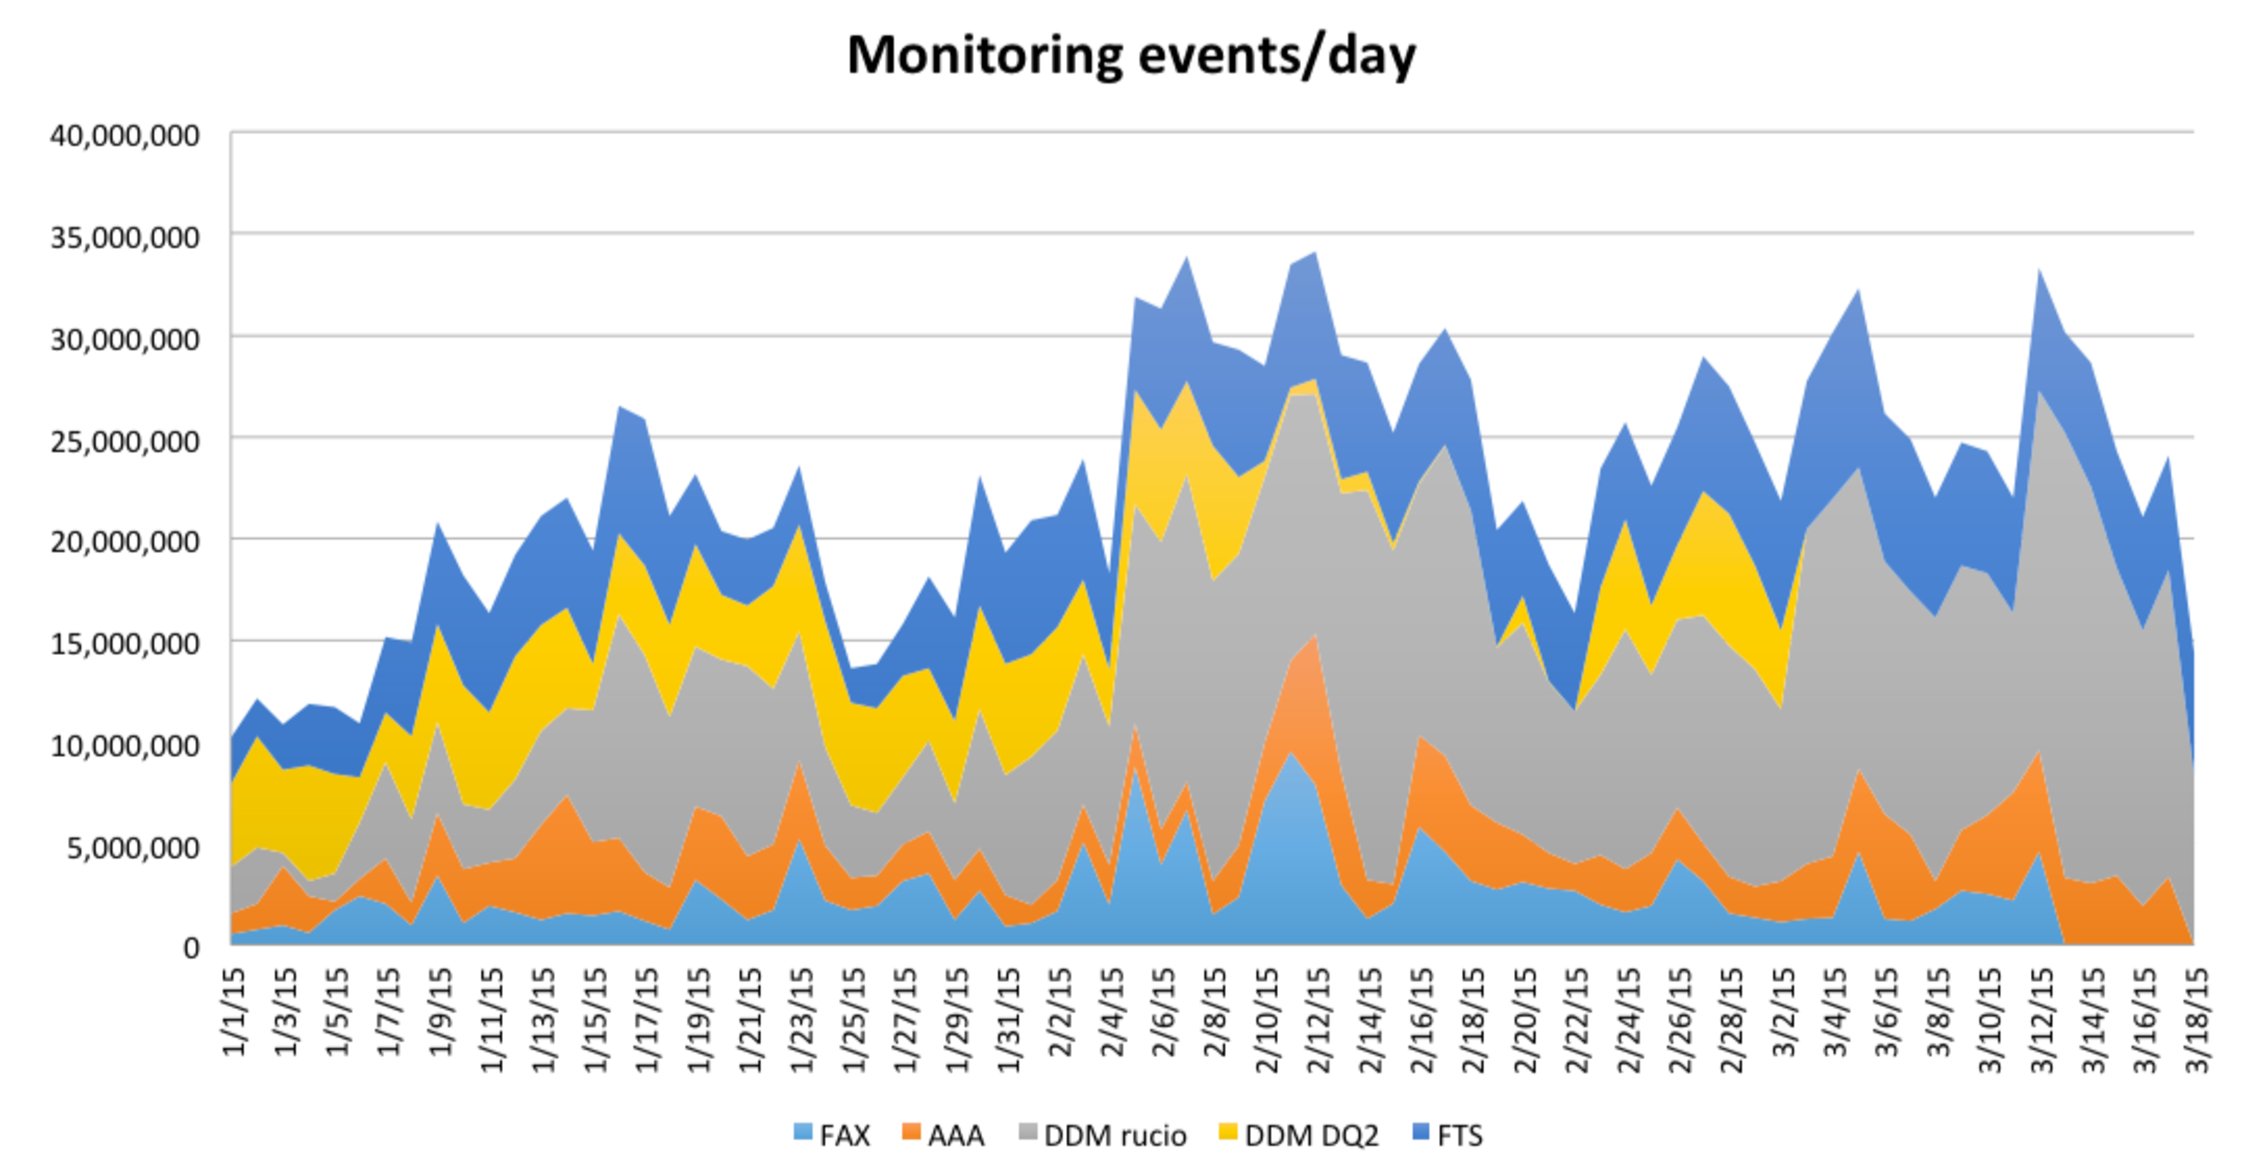
\includegraphics[width=120mm]{./Figures/wdt_volume.pdf}
  \caption{\small Daily volume of monitoring events for WDT dashboards.}\label{fig:wdt}
\end{figure}

\subsection{Towards a new approach for data store and processing} 

The current ED architecture relies on an Oracle database to store, to process
and to serve the monitoring data. Raw monitoring events are archived in tables
for several years, periodic PL/SQL jobs run at regular interval (10 minutes) to
transform the fresh raw data into summarized time-series statistics and feed
them in dedicated tables, from where they are exposed to the web-framework for
user visualization. For data intensive use cases, such as WDT, this approach
has several limitations. Scalability is difficult to achieve, PL/SQL execution
time fluctuating from tens of seconds to minutes as a consequence of the input
rate spikes, affecting user interface latency. Advanced processing algorithms
are complex to implement in PL/SQL within the dashboard 10 minutes time
constraint, and reprocessing of the full raw data can take days or weeks.
Moreover, the other dashboard components involved in data collection,
pre-processing and insertion are suffering from fragility and complexity,
leading to higher maintenance and operational costs and human faults.
Considering the foreseen increase in the WLCG monitoring data volume and
variety of monitoring events for the upcoming LHC runs, data store and
processing technologies which scale horizontally by design, such as Hadoop, are
suitable candidates for the evolution of the monitoring infrastructure. 
%The adoption of such technology requires a careful evaluation and the next
%sectiosn present the investiagtion done to esablish the best technology stack
%for the WLCG use case.
 

%\subsection{Requirements for the new architecture}

%The Monitoring section of the Support for Distributed Computing ( SDC) group, at the CERN IT department, is working on the research, the design and the development of the new data store and analytics platform for the evolution of the WLCG monitoring, able to cope with the scalability, flexibility and fault-tolerance requirements foreseen in the long-term WLCG scenario. 


%Requirements: Scalability/Simplicity/Mainstream

\section{The \textit{lambda} architecture}

In recent years, the challenge of handling a big volume of data has been taken
on by many companies, particularly in the internet domain, leading to a full
paradigm shift on data archiving, processing and visualisation. A number of new
technologies have appeared, each one targeting specific aspects on big-scale
distributed data-processing. All these technologies, such as batch
computation systems (e.g. Hadoop) and non-structured databases, can handle very
large data volumes with little cost but with serious trade-offs. The goal is to
architect a new platform in a tool-chain approach building on the most
appropriate technologies and computing techniques for the WLCG use case.

In this direction, the lambda architecture, presented by Marz in \cite{lambda} and successfully adopted by companies such as Twitter for data analysis, identified 3 main components to build a scalable and reliable data processing system:
\begin{itemize}
\item  the \textbf{batch layer}, to store a steadily growing dataset providing the ability to compute arbitrary functions on it;
\item  the \textbf{serving layer}, to save the processed views, using indexing techniques to make them efficiently query-able;
\item  the \textbf{real-time layer} able to perform analytics on fresh data with incremental algorithms to compensate for batch-processing latency. 
%Moreover, the real-time analytics layer can be used as input for active-reaction, adopting classical pattern matching approach to detecting errors and failures on the stream of monitoring events promptly. 
\end{itemize}

%\begin{figure}
%  \centering
%  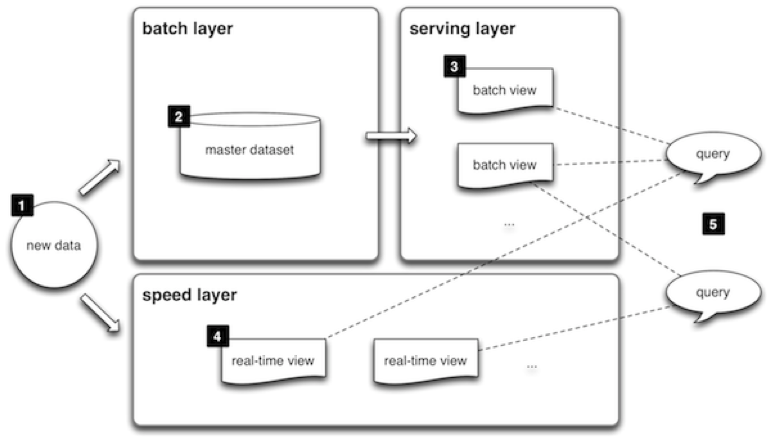
\includegraphics[width=60mm]{./Figures/lambda.png}
%  \caption{\small Sketch of the Lambda architecture, from (ref).}\label{fig:Lambda}
%\end{figure}

\subsection{Difference between WDT and the classic lambda use case}

In the classic lambda application each monitoring event only contributes to the
most recent view (e.g. a web server user access for a web analytics application
only affects the user count in the last time bin). For the WLCG monitoring use
case, this is not true. A monitoring event, such as a completed file transfer
lasting several hours from WLCG site A to site B, contributes also to several
time bins in the past, so that the information about the average traffic from
site A to site B has to be updated accordingly with the new monitoring
information. Without this initial hypothesis, the merging of batch and
real-time processing becomes more complex, as discussed in section 3.

\section{The new data store and analytics platform for WLCG monitoring}

The new data store and analytics platform for WLCG monitoring is presented in
Figure \ref{fig:narch} and it builds on a number of existing technologies and
tools in order to promote mainstream solutions and to minimize in-house code
development. The WLCG monitoring problem has been treated as a pure analytics
scenario where the driving concepts, as by the lambda principles, are to
collect and to store the raw data, to minimize pre-processing and to concentrate
analysis and transformation on the same framework with batch and real-time
components. 

\begin{figure}
  \centering
  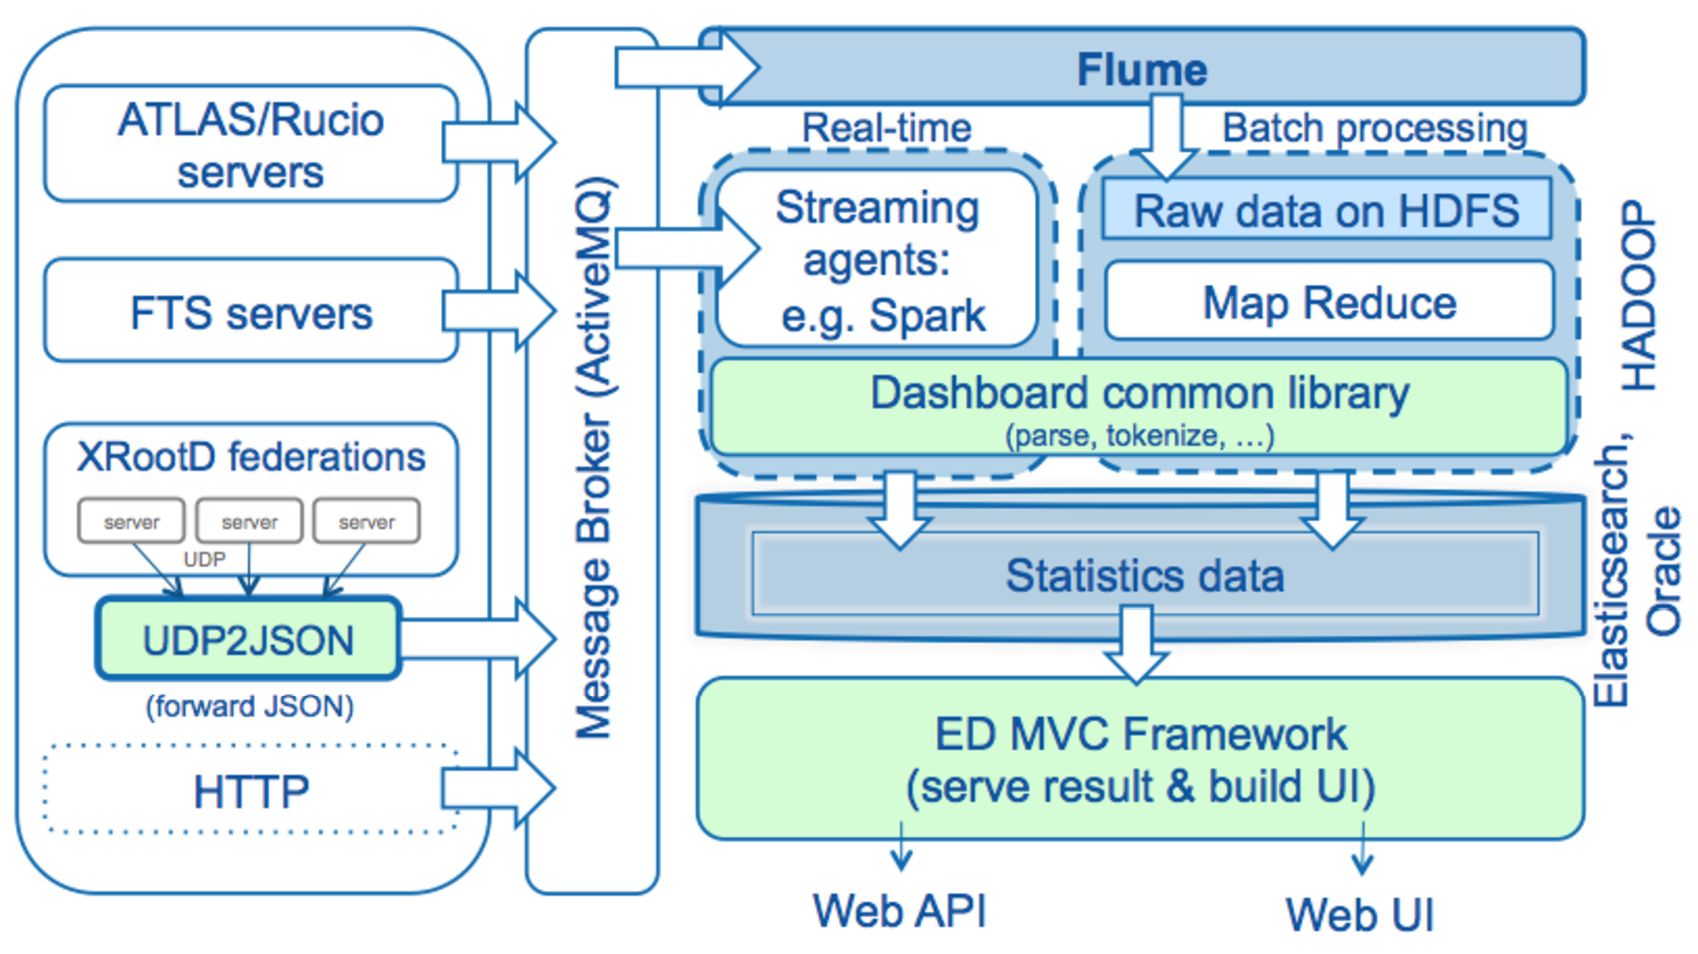
\includegraphics[width=120mm]{./Figures/new_arch.pdf}
  \caption{\small The new data analytics platform for WLCG monitoring.}\label{fig:narch}
\end{figure}

\subsection{Data transport: Message Broker}

The transport layer plays a key role in the new monitoring architecture.
Firstly, it decouples the producer and the consumer of the monitoring data.
Given that the information is produced by a variety of heterogeneous
applications and services in WLCG, this is a fundamental part of the system
functionality. Secondly, it allows multiple consumers to use the same data via
on-demand public/subscribe API. This situation is often the case for monitoring
data, which is also being used by LHC experiment specific frameworks. Thirdly,
the architecture can rely on message brokers as a service provided by the CERN
IT infrastructure. Currently, the broker technology used is ActiveMQ and the
monitoring events are reported as JSON records via the STOMP protocol.  A
possible future evolution is to explore tools such as Apache Kafka, a
specialized broker which improves the handling of big data volumes and works at
a higher data rate.

\subsection{Data collection: Apache Flume}

Apache Flume is used as the data collector agent. It receives monitoring events
from the transport layer and creates HDFS files in the archive layer for later
processing. It replaces a custom collector previously developed for the ED
framework, providing better performance and reliability. Flume connects to the
brokers using the standard JMS source and writes to the storage layer via the
standard HDFS sink.

\subsection{Batch processing: Apache Hadoop}

Hadoop is a distributed processing framework which allows the computation of
large data sets on computer clusters built from commodity hardware. Initially
focused mainly on batch-processing via the MapReduce primitives
\cite{mrgoogle}, modern Hadoop supports multiple processing technology, such as
Apache Spark.  MapReduce is the de-facto standard for batch processing and its
computation paradigm fits extremely well with the WDT use case, as presented in
section 4.  WDT batch-processing is implemented as periodic MapReduce jobs
running on the Hadoop infrastructure provided from CERN IT. The job algorithm
is stateless and idempotent, the full data set which can contribute to the
results (e.g. 3 days of data) being re-processed at each run. Job results are
written into the serving layer (i.e. Oracle table), which is then used to build
the web visualization. Moreover, WDT jobs also support Apache Spark
\cite{spark} as a processing framework. Spark is a modern distributed processing
technology, running on Hadoop or on standalone clusters, which improves the
MapReduce paradigm with a better in-memory computational model. In addition, it
also supports data streaming, which is useful in a lambda architecture to limit
code differences between batch and real-time. This flexibility is achieved via
the common WDT library presented below, which abstracts shared functionalities
and algorithms.


\subsection{Real-time processing: Spark streaming and Esper} 

Spark provides a streaming API for distributed processing of event streams.  A
continuous flow of data is divided into micro-batches (e.g. 10 seconds of events)
which can then be processed as if they were local data sets via standard Spark
in-memory primitives. Spark streaming jobs have been implemented to compute WDT
statistics on fresh monitoring events via an incremental algorithm.  Being
incremental hence not idempotent, special care is required in handling event
duplication and multiple processing, leading to a more error prone computation.
For this reason, and as by the lambda principles, the results from the
streaming jobs are continuously overwritten by the batch processing at each run
(e.g. every hour). Moreover, WDT streaming jobs were also implemented using
the open source event processing library Esper \cite{esper}. Compared with the basic Spark
primitives, Esper SQL-like language offers much more advanced controls in
processing streams over time.  For the WDT use case, where a basic map/reduce
paradigm fits the algorithm, the raw Spark primitives were preferred, but Esper
remains a valid option for other WLCG monitoring use cases when more advanced
processing is required. A possible evolution in this direction is to
investigate Esper as an embedded Spark streaming operator.
 

\subsection{Archiving: HDFS} 

The Hadoop framework is built on the Hadoop Distributed File System (HDFS) and
executes I/O operations on it. HDFS is designed for large data files, in the
order of GigaBytes in size. The data is broken into blocks and replicated
across multiple hosts in the cluster. This guarantees scalability on commodity
hardware, fault tolerance and high throughput. HDFS is data format independent,
it supports multiple data representations, from simple text to structured
binary. Section 4 presents the data format evaluation performed for the WDT use
case.

\subsection{The Dashboard Common library}
A common drawback of the dual processing nature of the lambda architecture is the
code duplication in the real-time and the batch processing layer. In order to
limit this effect a Java library has been developed to abstract the
common functionalities for the WDT use case. The library provides data parsing,
supporting marshalling and un-marshalling in several formats, such as JSON, CSV,
Avro, and also provides data validation and compression. Most importantly, it implements
the algorithm to emit key-value pairs for each monitoring events received. The
library played a major role in porting the WDT jobs to different processing
technologies (e.g. MapReduce, Spark) with minimal code change.

\subsection{The serving layer}

With the data archiving and processing delegated to the other components,
the serving layer is solely responsible for serving the computed statistics to
the ED web framework. In light of this simplified
requirement, for the WDT use case the serving layer can be easily implemented
via relational databases as well as by non-relational technology. In the new data analytics platform
the serving layer is still implemented using an Oracle database provided from
CERN IT database service. A promising investigation, still ongoing, is pointing at
Elasticsearch as a particularly good candidate to replace the current database.

\section{Implementation of WDT analytics on the new platform}
 
The current architecture uses PL/SQL procedures for aggregating and computing raw data into statistics with different time period granularities and stores them into a statistics table. WLCG data servers can produce monitoring logs at 1 kHz, with such a rate that the PL/SQL procedure cannot cope with the overwhelming amount of data, which takes over ten minutes to process every ten minutes worth of data. The new analytics platform relies on Hadoop and its MapReduce framework to overcome the current latency and scalability issues. MapReduce is a programming paradigm that was designed to remove the complexity of processing data that are geographically scattered around a distributed infrastructure \cite{mrgoogle}. It hides the complexity of computing in parallel, load balancing and fault tolerance over an extensive range of interconnected machines. There are two simple parallel methods, \textit{map} and \textit{reduce}, which are predefined in the MapReduce programming model and are user-specified methods that are used to develop the analytics platform.

%\par


\begin{figure}
  \centering
  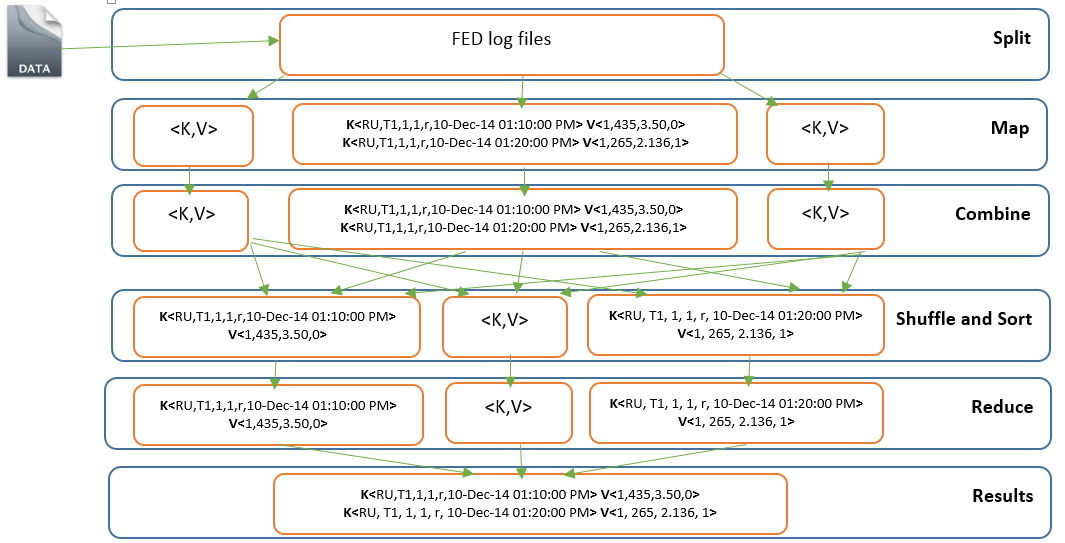
\includegraphics[width=100mm]{./Figures/MR.png}
  \caption{\small MapReduce computations diagram.}\label{fig:mapframe}
\end{figure}

\vspace{5mm}

Figure \ref{fig:mapframe} shows an how WDT MapReduce jobs are carried out by each component within the MapReduce framework: 

\begin{enumerate}
 \item A \textit{splitter} will split the monitoring data into lines and feed them into mappers.
 \item A \textit{mapper} will process the line; breaking them into the time bins in which they belong and calculating the transfer matrices. %(e.g. transferred bytes, active files, finished files, active time, etc.). 
Finally, it will emit key/value pairs for each time bin.
 \item A \textit{combiner} will run after each map task and aggregate a map output result, decreasing the number of metrics sent to the reducer.
 \item The output of the combiner is then shuffled and transferred to a reducer that is responsible for processing the key  and carrying out the final summing.
 \item A \textit{reducer} will aggregate and output the final results.
\end{enumerate}

\subsection{Data representation}
In the current architecture the data are partitioned in HDFS, as shown in Figure \ref{fig:dstructure}, for efficient processing, as this will support the processing of data by specified date ranges.

\begin{figure}[!htb]
\centering
\begin{minipage}{.5\textwidth}
\centering
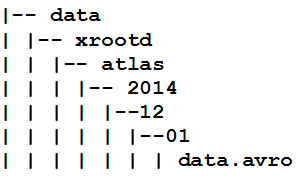
\includegraphics[width=60mm]{./Figures/dstructure.png}
\caption{\small HDFS data partitioning.}\label{fig:dstructure}
\end{minipage}%
\begin{minipage}{0.5\textwidth}
\centering
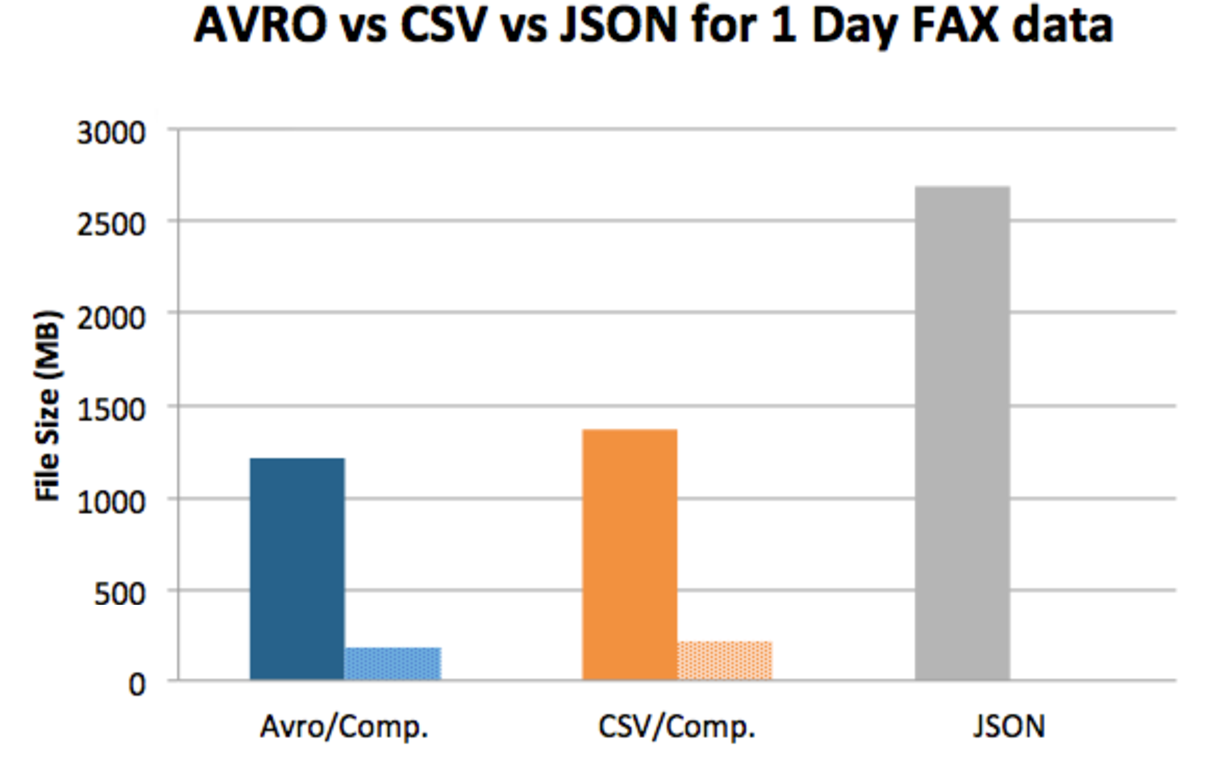
\includegraphics[width=60mm]{./Figures/format_plot.pdf}
\caption{\small Data format comparison.}\label{fig:format}
\end{minipage}
\end{figure}

Three different data formats were evaluated to store WDT monitoring data on HDFS: 
\begin{enumerate}
\item Avro is a data serialisation framework that serialises the data into a compact binary format, so that it can be transferred efficiently across the network.
\item Comma-Separated Value (CSV) is a table format that maps very well to the tabular data.
\item JavaScript Object Notation (JSON) is primarily a way to store simple object trees.
\end{enumerate}
\vspace{5mm}
Figure \ref{fig:format} shows data representing 1 (average) day of monitoring events for the ATLAS XRootD federation (FAX) on HDFS which occupies 1211 MBytes in Avro, 1367 MBytes in CSV and 2669 MBytes in JSON file format. 
%Figure \ref{fig:format} shows one day of data collected from the ATLAS XRootD federation (FAX), which clusters Tier-1, Tier-2 and Tier-3 storage resources together into a common namespace and allows remote accessibility from geographically separated sites
As expected, the Avro format is more compact than CSV and JSON. This is because the binary version of Avro is used, whereas CSV comprises human readable comma-separated columns and JSON contains tree structured data. The JSON format took a larger space because it holds both column name and data, whereas CSV only holds the data that are separated by comma. This has resulted in a 122.21\% increase in volume for JSON data and a 12.88\% increase in volume for CSV data compared with Avro, while there is a 96.85\% increase in volume for JSON data compared with CSV. The data were also compressed using the Snappy compression library, which is very fast but the compaction ratio is very low compared with other libraries. Again, compressed Avro data takes up much less room than the CSV as there is a 20.90\% increase in volume. It can be seen that compressed data took over 5 times less space than uncompressed. The test results, combined with the additional benefits of being schema-based and its multi-language support, make Avro the preferred option for the WDT use case.  
%\begin{figure}
 % \centering
 % 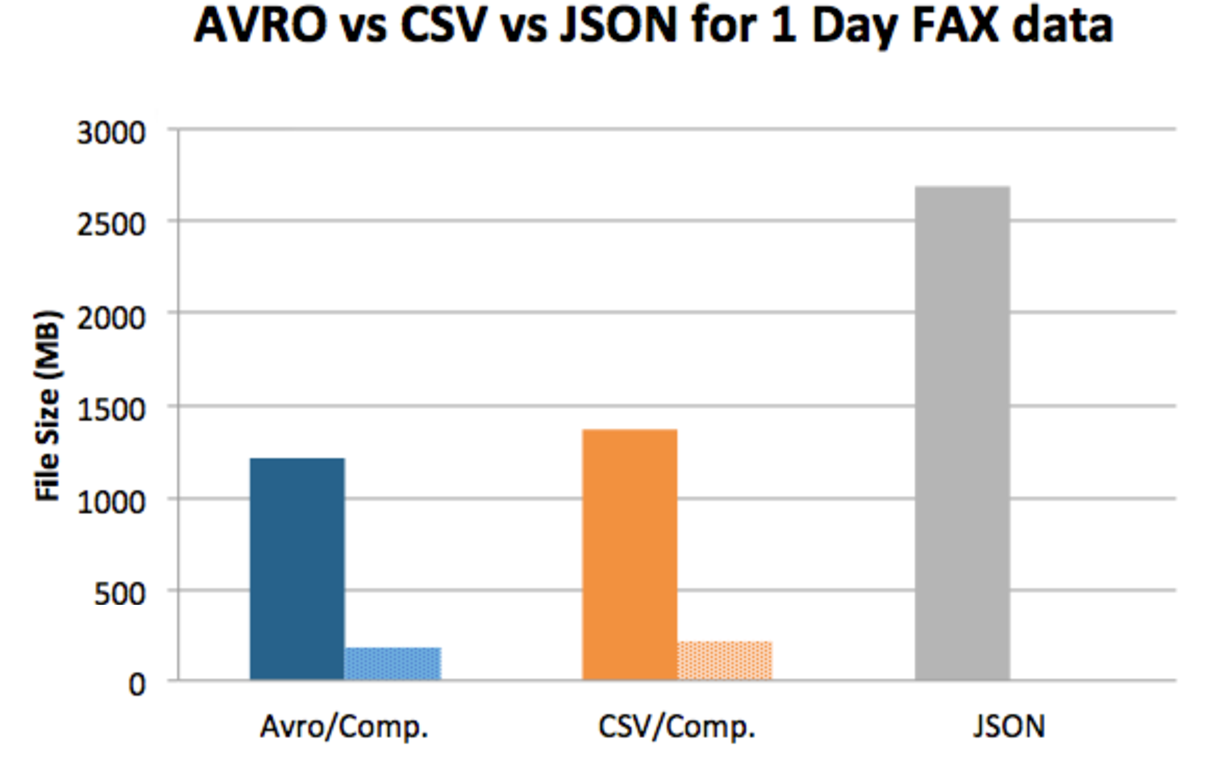
\includegraphics[width=60mm]{./Figures/format_plot.pdf}
 % \caption{\small Data format comparison.}\label{fig:format}
%\end{figure}

\section{Performance results for WDT computation on the new platform}
%Avro, CSV , JSON
%Partitioning
In order to evaluate the execution time of jobs on the new platform architecture, it was decided to compute FAX dataset by days, ranging from: 1 day, 3 days, 7 days and 21 days. Jobs were submitted a few times for each dataset  in order to capture an average performance time. The performance measurements were carried out on a heterogeneous Hadoop cluster that consisted of fifteen nodes (8 nodes: 32 cores/64GB, 7 nodes: 4 cores/8GB).

%and their specifications were as shown in Table \ref{table:1}.

%\begin{table}[h!]
%\centering
%\caption{Cluster specifications}
%\begin{tabular}{ l | c }
%  \hline  
%	 No.Nodes & Specifications \\ \hline
%  8 nodes & 32 cores/64GB \\
%  7 nodes & 4 cores/8GB  \\
%  \hline  
%\end{tabular}
%\label{table:1}
%\end{table}
The main result, as presented by the plot in Figure \ref{fig:mr}, is that the jobs were able to successfully process all data ranges in at most just few minutes. This result alone satisfies the WDT requirement of updating monitoring information every 10 minutes with fresh data and allows for re-processing of years of monitoring logs. Moreover, it demonstrates the scalability of the system over different data volumes.
%In Figure \ref{fig:mr}, the comparison between the execution time and data input size of compressed and uncompressed Avro, CSV and JSON jobs can be seen. 
In general, computation of uncompressed data was faster than compressed data with the exception of JSON data as it is very large compared to other formats. It is understandable why compressed data were slow to process as the data will need to be uncompressed before processing and will therefore add additional overheads to the computation time. Although uncompressed Avro and CSV jobs were fast, the CSV appears to be the fastest.
% This observation contradicted previous experiments conducted on another cluster as Avro clearly outperformed the CSV in this earlier study. 
This can be explained by the computing limitation of the cluster due to its heterogeneous setup.
%  It was expected that the processing time for CSV data would be longer than for Avro data because use of CSV format adds an extra overhead for parsing data into appropriate data types for computations, whereas Avro is not required to parse data due to the fact that data are accompanied with a schema. However, this was found not to be the case on this cluster and the logical explanation is that the nodes are unbalanced as 8 of the total 15 nodes have a high specification and 7 are average. Therefore, CSV data could have been distributed to the high performance nodes, whereas the Avro data could have been delivered to the average nodes, resulting in the parsing and computing of CSV data at a faster speed than for the Avro data.

It should be noted that largely there is not much difference between the execution time of the process on the 1 day dataset compared with the 21 day dataset, while being many times bigger in size. This demonstrates the scalability of the Hadoop system, which distributes the computation across several nodes. Nevertheless, there is always a fixed overhead added to the job for finding appropriate resources and submitting them. Even though the job is split into multiple map tasks and sent to data nodes where the data reside in order to reduce the movement of large data files over the network, the intermediate results of these tasks still need to be shuffled and shifted around to reducers (most likely to different nodes) \cite{mrgoogle}. This could create a bottleneck in the network, so in order to minimise this issue, it was decided to compress the intermediate results, improving by $\sim2$ seconds the time for transferring them to the reducer nodes. This results were obtained using the MapReduce version of the WDT jobs, but comparable measurements have been observed using Apache Spark for batch processing.

%\subsection{MR performance}
\begin{figure}
  \centering
  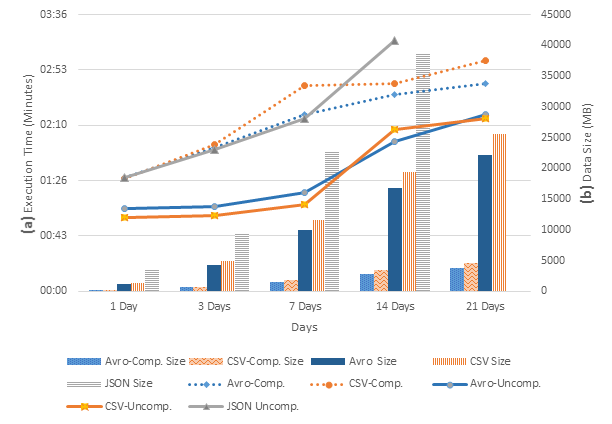
\includegraphics[width=140mm,height=80mm]{./Figures/mp_perf.png}
  \caption{\small Computation of Compressed/Uncompressed Avro, CSV and JSON files over different date ranges. The primary axis (a) shows the execution time that is being represented by lines, whereas the secondary axis (b) represents the input data size in Megabytes (MB) which is represented by bars.}\label{fig:mr}
\end{figure}

\section{Conclusion and next steps}

The new data store and analytics platform presented in this paper is a
scalable, simplified and effective solution for WLCG activities monitoring. It
builds on a set of mainstream technologies, and uses the lambda architecture
principles to assemble them in a reliable and effective way. The performance
test results show how the MapReduce/Spark approach outperforms the current
system and that it can scale horizontally to support the increase of the
volume and the variety of WLCG monitoring events in the upcoming years of LHC data
taking.

The next steps are to complete the migration of the WDT dashboards to the new
architecture and to evaluate the new platform for the other Experiment
Dashboard applications. Further investigation into the serving layer technology
and the optimal strategy for integrating batch and real-time data processing is
ongoing. 






%\addcontentsline{toc}{chapter}{Optimising lambda architecture using Apache Spark technology}
\chapter{Optimising lambda architecture using Apache Spark technology} \label{spark-eva}

%\section{Motivations} \label{Motivations}

\section{Introduction} \label{spark-intro}
\section{Summary} \label{spark-summ}




%\addcontentsline{toc}{chapter}{Optimising real-time processing with built-in intelligence}
\chapter{Exploiting data popularity to model the evolution of data management using real-time processing and Machine Learning} \label{ml-real}

%\section{Motivations} \label{Motivations}

\section{Introduction} \label{ml-intro}
\section{Summary} \label{ml-summ}






%\addcontentsline{toc}{chapter}{Conclusions}
\chapter{Conclusions and Future Work} \label{concl-future}

%\section{Motivations} \label{Motivations}

\section{Conclusions} \label{conclusions}
\section{Future Work} \label{future-work}






\appendix
\appendixpage
\addappheadtotoc

\renewcommand{\thesection}{A.\arabic{section}}
\renewcommand\thefigure{\thesection}
\renewcommand\thetable{\thesection}

\section*{References}

\bibliography{PhDThesis}
\bibliographystyle{unsrt}

\end{document}
